% This is part of Un soupçon de mathématique sans être agressif pour autant
% Copyright (c) 2012
%   Laurent Claessens
% See the file fdl-1.3.txt for copying conditions.


% This is part of Un soupçon de mathématique sans être agressif pour autant
% Copyright (c) 2012-2014
%   Laurent Claessens
% See the file fdl-1.3.txt for copying conditions.


\usepackage{etex}
\usepackage{ifthen}
%\usepackage{pdfsync}       % This package is obsolete : compile with pdflatex -synctex=1 instead.

\usepackage{latexsym}
\usepackage{amsfonts}
\usepackage{amsmath}
\usepackage{amsthm}
\usepackage{amssymb}
\usepackage{bbm}
\usepackage{mathrsfs}           
\usepackage{mathabx}           % Pour \divides

\usepackage{framed} % pour oframed
\usepackage{wrapfig}

\usepackage{calc}   % Les dépendances de phystricks si on n'utilise que le pdf.
%\usepackage{pstricks,pst-eucl,pstricks-add,calc,pst-math}   % Les dépendances de phystricks. Peut être qu'il faut ajouter catchfile


% Les dépendances de phystricks en mode Tikz
\usepackage{tikz}
\usepackage{calc}
\usetikzlibrary{calc}
\usetikzlibrary{patterns}

\usetikzlibrary{external}
\tikzexternalize
%\newcommand{\tikzsetnextfilename}[1]{}
\newcounter{defHatch}
\newcounter{defPattern}
\setcounter{defHatch}{0}
\setcounter{defPattern}{0}


\usepackage{graphicx}                   % Pour l'inclusion d'image en pfd.

%\newcommand{\EpsOrPdfincludegraphics}[2][]{%
%        \ifpdf
%            \includegraphics[#1]{#2.png}
%        \else
%            \includegraphics[#1]{#2.eps}
%        \fi
%        }

\usepackage{subfigure}

\usepackage{fancyvrb}
\usepackage{stmaryrd}       % Pour le \obslash
\usepackage{xstring}        % Utilisé pour les références vers wikipédia
\usepackage{cases}
\usepackage{lscape}         % pour l'environnement landscape, utilisé dans la correction corr0076.tex
\usepackage{multicol}
\setlength{\columnseprule}{0.5pt}
\usepackage{import}         % Pour le hack qui sert à inclure GeomAnal

% TODO : n'en utiliser qu'un
\usepackage[normalem]{ulem}     % Pour le barré, commande \sout
\usepackage{soul}       % Pour le barré, commande \st

\usepackage[all]{xy}

\let\second\undefined      % le paquet amthabx définit \second
\let\degree\undefined       % le paquet amthabx définit \degree
%\usepackage[cdot,thinqspace,amssymb]{SIunits} 
\usepackage[parse-numbers=false,binary-units=true,detect-all=true,per-mode=symbol]{siunitx} 
\newcommand{\unit}[2]{\SI{#1}{#2}}
 % L'option amssymb sert à éviter un conflit avec la commande \square de amssymb. Note qu'elle n'est plus accessible. Si tu en as besoin, faudra RTFM
%ftp://ftp.belnet.be/packages/ctan/macros/latex/contrib/SIunits/SIunits.pdf

\usepackage[nottoc]{tocbibind}
\usepackage[numbers]{natbib}

%%%%%%%%%%%%%%%%%%%%%%%%%%
%
%   Trucs mathématiques
%
%%%%%%%%%%%%%%%%%%%%%%%%

% ENSEMBLES DE NOMBRES
\newcommand{\eA}{\mathbbm{A}}
\newcommand{\eC}{\mathbbm{C}}
\newcommand{\eD}{\mathbbm{D}}
\newcommand{\eE}{\mathbbm{E}}
\newcommand{\eF}{\mathbbm{F}}
\newcommand{\eG}{\mathbbm{G}}
\newcommand{\eH}{\mathbbm{H}}
\newcommand{\eK}{\mathbbm{K}}
\newcommand{\eL}{\mathbbm{L}}
\newcommand{\eM}{\mathbbm{M}}
\newcommand{\eN}{\mathbbm{N}}
\newcommand{\eP}{\mathbbm{P}}
\newcommand{\eQ}{\mathbbm{Q}}
\newcommand{\eR}{\mathbbm{R}}
\newcommand{\eZ}{\mathbbm{Z}}

% ENSEMBLES de fonctions
\newcommand{\aL}{\mathcal{L}}       % Les applications linéaires
\newcommand{\aC}{\mathcal{C}}       % Les fonctions C^1, C^2 etc



\newcommand{\mF}{\mathcal{F}}
\newcommand{\mC}{\mathcal{C}}
\newcommand{\mG}{\mathcal{G}}
\newcommand{\mI}{\mathcal{I}}
\newcommand{\mL}{\mathcal{L}}
\newcommand{\mS}{\mathcal{S}}   % Utilisé pour l'espace des fonctions Schwartz
\newcommand{\mZ}{\mathcal{Z}}


\newcommand{\mtu}{\mathbbm{1}}              % La matrice unité

\DeclareMathOperator{\val}{val}     % valuation d'un polynôme
%\DeclareMathOperator{\opp}{opp}    % Les nombres négatifs


%\newcommand{\efrac}[2]{\frac{ \displaystyle #1 }{\displaystyle #2 }}
%%%%%%%%%%%%%%%%%%%%%%%%%%
%
%   Numérotations en tout genre
%
%%%%%%%%%%%%%%%%%%%%%%%%

\setcounter{tocdepth}{2}        % Profondeur de la table des matières
\setcounter{secnumdepth}{2}     % Profondeur dans le texte

\renewcommand{\thesubsection}{\thesection.\alph{subsection}}

%%%%%%%%%%%%%%%%%%%%%%%%%%
%
%   Les lignes magiques pour le texte en français.
%
%%%%%%%%%%%%%%%%%%%%%%%%

\usepackage[utf8]{inputenc}
\usepackage[T1]{fontenc}

\usepackage{listingsutf8}
%\lstset{language=python,basicstyle=\footnotesize,tabsize=3,numbers=left,numberstyle=\tiny,frame=single,commentstyle=\ttfamily\color[rgb]{0,0,0.5},stringstyle=\color[rgb]{0,0.5,0},title=\lstname,inputencoding=utf8/latin1}
\lstset{language=python,basicstyle=\footnotesize,tabsize=3,frame=single,commentstyle=\ttfamily\color[rgb]{0,0,0.5},stringstyle=\color[rgb]{0,0.5,0},title=\lstname,inputencoding=utf8/latin1}

\usepackage[fr]{exocorr}
\usepackage{textcomp}
\usepackage{lmodern}
\usepackage[a4paper,margin=2cm]{geometry} 
\usepackage[english,frenchb]{babel}


\usepackage{hyperref}                           %Doit être appelé en dernier.
\hypersetup{
colorlinks=true,
linkcolor=blue,
urlcolor=magenta,     % couleur des url
filecolor=magenta   % couleur des textes qui sont des liens
}

% Il me semble que cette commande doit être définie après l'appel à Babel.
\newcommand{\Ieme}{\up{\lowercase{ième}}\xspace}

%%%%%%%%%%%%%%%%%%%%%%%%%%
%
%   Les théorèmes et choses attenantes
%
%%%%%%%%%%%%%%%%%%%%%%%%


\newcounter{numtho}
\newcounter{numprob}

\makeatletter
\@addtoreset{numtho}{chapter}
%\@addtoreset{CountExercice}{chapter}
\@addtoreset{chapter}{part}
\makeatother

\newlength{\EnvSpace}
\setlength{\EnvSpace}{9pt}      % C'est la distance que je veux mettre avant et après les théorèmes, remarques, etc.

\newtheoremstyle{MyTheorems}%
        {\EnvSpace}{\EnvSpace}%
        {\itshape}%
        {}%
        {\bfseries}{.}%
        {\newline}%
        {}%
\newtheoremstyle{MyExamples}%
        {\EnvSpace}{\EnvSpace}%
        {}%
        {}%
        {\bfseries}{.}%
        {\newline}%
        {}%
\newtheoremstyle{MyRemarks}%
        {\EnvSpace}{\EnvSpace}%
        {}%
        {}%
        {\bfseries}{.}%
        {\newline}%
        {}%

%\theoremstyle{MyExamples}   %\newtheorem{exemple}[numtho]{Exemple}      % Pour unification, ne plus utiliser
%                            \newtheorem{example}[numtho]{Exemple}
\newcounter{CounterExample}
\renewcommand{\theCounterExample}{\thechapter.\arabic{CounterExample}}

% J'ai décidé de ne plus numéroter les choses encadrées. 8 avril 2014
\newenvironment{example}{\vspace{\EnvSpace}\refstepcounter{numtho}\noindent{\bf Exemple}\\\nopagebreak}{\phantom{a}\hfill $\triangle$\vspace{\EnvSpace}}
\newenvironment{Aretenir}{\refstepcounter{numtho}\begin{oframed}\noindent{\bf À retenir}\newline}{\end{oframed}\vspace{\EnvSpace}}
\newenvironment{Aprojeter}{\clearpage\phantom{a}\vfill}{\vfill\newpage}
\newenvironment{definition}[1][]{\refstepcounter{numtho}\begin{oframed}\noindent{\bf Définition}#1\newline}{\end{oframed}\vspace{\EnvSpace}}
\newenvironment{propriete}{\refstepcounter{numtho}\begin{oframed}\noindent{\bf Propriété}\newline}{\end{oframed}\vspace{\EnvSpace}}

\newenvironment{Enmini}{\begin{oframed}\noindent{\bf Mini résumé}\newline}{\end{oframed}\vspace{\EnvSpace}}
% Ce bout de code provient de BrunoJ
% https://brunoj.wordpress.com/2009/10/08/latex-the-framed-minipage/
\newsavebox{\fmbox}
 \newenvironment{fmpage}[1]
 {\begin{lrbox}{\fmbox}\begin{minipage}{#1}}
     {\end{minipage}\end{lrbox}
     \fbox{\usebox{\fmbox}}
 }

\theoremstyle{MyRemarks}    \newtheorem{remark}[numtho]{Remarque}

                \newtheorem{amusement}[numtho]{Amusement}
                \newtheorem{erreur}[numtho]{Error}
                \newtheorem{probleme}[numprob]{\fbox{\bf Problèmes et choses à faire}}


\theoremstyle{MyTheorems}
\newtheorem{lemma}[numtho]{Lemme}
\newtheorem{corollary}[numtho]{Corollaire}
\newtheorem{theorem}[numtho]{Théorème}      
\newtheorem{proposition}[numtho]{Proposition}      


\renewcommand{\thenumtho}{\thechapter.\arabic{numtho}}
% La numérotation des équations change dans les corrigés
\renewcommand{\theequation}{\thechapter.\arabic{equation}}
\renewcommand{\theCountExercice}{\arabic{CountExercice}}       % Ce compteur est défini dans SystemeCorr.sty
\newcommand{\defe}[2]{\textbf{#1}\index{#2}}

\renewcommand{\theenumi}{(\alph{enumi})}
\renewcommand{\theenumii}{(\alph{enumi}\arabic{enumii})}

\renewcommand{\labelenumi}{\theenumi}
\renewcommand{\labelenumii}{\theenumii}

\newcommand{\justification}{ {\small \begin{center}    Attention : vous devez laisser sur votre feuille les traces de vos recherches et les étapes intermédiaires de vos calculs !    \end{center}}}
    

    % L'une des deux est avec le nom et l'autre sans.
    \newenvironment{feuilleDS}[1]{\noindent Nom, Prénom : \begin{center}\large #1\\\justification\end{center}\setcounter{CountExercice}{0}  }{\clearpage}
    %\newenvironment{feuilleDS}[1]{\begin{center}\large #1\\\justification\end{center}\setcounter{CountExercice}{0}  }{\clearpage}


    \newenvironment{feuilleExo}[1]{\newpage\begin{center}\large #1\end{center}\setcounter{CountExercice}{0}  }{\clearpage}
    %\newenvironment{feuilleExo}[1]{\begin{center}\large #1\end{center}\setcounter{CountExercice}{0}  }{}

        
        \newcounter{numactivmentale}
        \setcounter{numactivmentale}{0}
        \newcounter{numExoMental}
        \setcounter{numExoMental}{0}
        \newenvironment{MentalActivity}{\setcounter{numExoMental}{0}\newpage\refstepcounter{numactivmentale}\section{Activité mentale \arabic{numactivmentale}}}{\newpage\hphantom{jj}\vfill\large C'est tout pour aujourd'hui\vfill\newpage}
        \newenvironment{mental}{\refstepcounter{numExoMental}\newpage\begin{center}\fbox{\huge Activité mentale \arabic{numactivmentale}}\\\huge Question \arabic{numExoMental}\end{center}\huge\vfill}{\vfill}


\newcommand{\enteteInterro}[3]{
    \begin{center}
        #1\\
        Intérogation #2, sujet #3
    \end{center}
    Nom, prénom, classe : \ldots\\
    \setcounter{CountExercice}{0}
}


%%%%%%%%%%%%%%%%%%%%%%%%%%
%
%   Les macros qui font des choses
%
%%%%%%%%%%%%%%%%%%%%%%%%

\newcommand{\mA}{\mathcal{A}}
\newcommand{\mO}{\mathcal{O}}
\newcommand{\mR}{\mathcal{R}}
\newcommand{\mT}{\mathcal{T}}
\newcommand{\mU}{\mathcal{U}}

\newcommand{\scal}[2]{ \langle #1,#2\rangle }

\newcommand{\tq}{\text{ tel que }}
\newcommand{\tqs}{\text{ tels que }}
\newcommand{\quext}[1]{ \footnote{\textsf{#1}}  }
\newcommand{\info}[1]{\texttt{#1}}
\newcommand{\vect}[1]{\overrightarrow{#1}}    % Cette macro est codée en dur dans phystricksDefVecteurAXDDGP et dans d'autres

\newcommand{\VarAbs}{\text{Var}_{\text{abs}}}
\newcommand{\VarRel}{\text{Var}_{\text{rel}}}

\newcommand{\normal}{\lhd}
\newcommand{\swS}{\mathscr{S}}          % L'ensemble des fonctions Schwartz

%\newcommand{\defD}{\mathscr{D}}     % Ensemble de définition d'une fonction
\newcommand{\defD}{D}                % Le D avec des croles était impossible à comprendre pour les élèves.

\newcommand{\Borelien}{\mathcal{B}\text{or}}       % Les boréliens
\newcommand{\tribA}{\mathcal{A}}            % Une tribu A
\newcommand{\tribB}{\mathcal{B}}            
\newcommand{\tribF}{\mathcal{F}}            % Une tribu F

\newcommand{\affE}{\mathcal{E}}            % Un espace affine E
\newcommand{\affF}{\mathcal{F}}            
\newcommand{\affG}{\mathcal{G}}            

\newcommand{\statS}{\mathcal{S}}            % Un modèle statistique
\newcommand{\partP}{\mathcal{P}}            % L'ensemble des parties d'un ensemble

\newcommand{\polyP}{\mathcal{P}}            % L'ensemble des polynômes

\newcommand{\dB}{\mathscr{B}}       % la distribution de Bernoulli
\newcommand{\dE}{\mathscr{E}}       % la distribution exponentielle
\newcommand{\dG}{\mathscr{G}}       % la distribution géométrique.
\newcommand{\dM}{\mathscr{M}}       % la distribution multinomiale
\newcommand{\dN}{\mathscr{N}}       % la distribution normale.
\newcommand{\dP}{\mathscr{P}}       % la distribution de Poisson.
\newcommand{\dT}{\mathscr{T}}       % la distribution de Student
\newcommand{\dU}{\mathscr{U}}       % la distribution uniforme

\newcommand{\hL}{\mathscr{L}}       
\newcommand{\cL}{\hL}           % Pour la partie Chafai

\newcommand{\modE}{\mathcal{E}}         % Le E des modules
\newcommand{\modF}{\mathcal{F}}         % Le F des modules
\newcommand{\hH}{\mathscr{H}}           % Le H des espaces de Hilbert

%%%%%%%%%%%%%%%%%%%%%%%%%%
%
%   Bibliographie, index et liste des notations
%
%%%%%%%%%%%%%%%%%%%%%%%%

\usepackage{makeidx}
\usepackage[nottoc]{tocbibind}      % Le paquetage qui fait en sorte que la biblio soit inclue correctement dans la table des matières.
\usepackage[refpage]{nomencl}
\renewcommand{\nomname}{Liste des notations}
%
%   Comment introduire des éléments dans l'index des notations.
%
% La liste des tags à mettre pour bien classer mes notations est :
% T     pour la topologie et théorie des ensembles
%
% La syntaxe est facile, par exemple 
%       $\SL(2,\eR)$\nomenclature[G]{$\SL(2,\eR)$}{Le groupe de matrices deux par deux de déterminant 1.}
%\renewcommand{\nomgroup}[1]{%
%    \ifthenelse{\equal{#1}{A}}{\item[\textbf{Algèbre}]}{}%
%    \ifthenelse{\equal{#1}{G}}{\item[\textbf{Géométrie}]}{}%
%    \ifthenelse{\equal{#1}{R}}{\item[\textbf{Théorie des groupes}]}{}%
%    \ifthenelse{\equal{#1}{P}}{\item[\textbf{Probabilités et statistique}]}{}%
%    \ifthenelse{\equal{#1}{Y}}{\item[\textbf{Analyse}]}{}%
%    \ifthenelse{\equal{#1}{M}}{\item[\textbf{Chaînes de Markov}]}{}%
%}

%%%%%%%%%%%%%%%%%%%%%%%%%%
%
%   DeclareMathOperator
%
%%%%%%%%%%%%%%%%%%%%%%%%

\DeclareMathOperator{\signe}{sgn}
\DeclareMathOperator{\Vol}{Vol}
\DeclareMathOperator{\Int}{Int}     % Intérieur d'un ensemble.
\DeclareMathOperator{\Ind}{Ind}     % l'indice d'un chemin en analyse complexe
\DeclareMathOperator{\Diam}{Diam}   
\DeclareMathOperator{\id}{Id}   
\DeclareMathOperator{\Graph}{Graph} 
\DeclareMathOperator{\pr}{\texttt{proj}}
\DeclareMathOperator{\dom}{dom}

\DeclareMathOperator{\Graphe}{Gr}
\DeclareMathOperator{\Spec}{Spec}   % spectre d'un opérateur
\DeclareMathOperator{\arctg}{arctg}
\DeclareMathOperator{\cotg}{cotg}
\DeclareMathOperator{\cosec}{cosec}
\DeclareMathOperator{\arcsinh}{arcsinh}

\DeclareMathOperator{\GL}{GL}   % le groupe linéaire
\DeclareMathOperator{\PGL}{PGL}   % le groupe projectif
\DeclareMathOperator{\SO}{SO}           
\DeclareMathOperator{\SL}{SL}           
\DeclareMathOperator{\PSL}{PSL}   % Le groupe modulaire SL(2,Z)/Z2
\DeclareMathOperator{\gO}{O}           
\DeclareMathOperator{\SU}{SU}           
\DeclareMathOperator{\gU}{U}           

\DeclareMathOperator{\Reel}{Re}        % La partie réelle d'un nombre complexe

\DeclareMathOperator{\Image}{Image}        % ... avec \Image qui donne l'image d'une fonction ou d'un opérateur.
\DeclareMathOperator{\rang}{rg}   
\DeclareMathOperator{\Kernel}{Ker}
\DeclareMathOperator{\Domaine}{Dom}
\DeclareMathOperator{\Span}{Span}
\DeclareMathOperator{\Hom}{Hom}
\DeclareMathOperator{\End}{End}     % L'ensemble des endomorphismes
\DeclareMathOperator{\tr}{Tr}       % la trace
\DeclareMathOperator{\Majorant}{Maj}
\DeclareMathOperator{\codim}{codim} % pour la codimension.
\DeclareMathOperator{\diam}{diam} % le diamètre d'un ensemble.

\DeclareMathOperator{\Var}{Var}     % Variance d'une variable aléatoire.
\DeclareMathOperator{\Fun}{\texttt{Fun}}     % Ensemble des applications d'un ensemble vers l'autre.
\DeclareMathOperator{\Cov}{Cov}     % la covariance.
\DeclareMathOperator{\gr}{gr}     % le groupe engendré
\DeclareMathOperator{\pgcd}{pgcd}     
\DeclareMathOperator{\ppcm}{ppcm}     
\DeclareMathOperator{\Frob}{Frob}     
\DeclareMathOperator{\Card}{Card}       % Le cardinal d'un ensemble.
\DeclareMathOperator{\Stab}{Stab}       % Le stabilisateur d'un point sous l'action d'un groupe.

\DeclareMathOperator{\Frac}{Frac}       % le corps des fractions d'un anneau
\DeclareMathOperator{\Aff}{Aff}         %  l'espace affine engendré

\newenvironment{subproof}{\begin{description}}{\end{description}}

\newcommand{\telque}{\vert\,}
\newcommand{\donc}{\Rightarrow}

\usepackage{mathtools}
\mathtoolsset{showonlyrefs}



\makeindex
\makenomenclature

\begin{document}

\corrPosition{1}
%\corrDraft{1}


% This is part of Un soupçon de mathématique sans être agressif pour autant
% Copyright (c) 2012
%   Laurent Claessens
% See the file fdl-1.3.txt for copying conditions.

\thispagestyle{empty}
\begin{center}
  \begin{minipage}{15cm}
    \hrule\par
    \vspace{2mm}
    \begin{center}
    \Huge \bfseries Un soupçon de mathématiques sans être agressif pour autant \par
    \end{center}
    \hrule\par
  \end{minipage}
\end{center}

\vspace{2cm}

\begin{center}
    Laurent \textsc{Claessens}\\
    \today\\
    Dernière version :\\
    \url{http://student.ulb.ac.be/~lclaesse/smath.pdf}
\end{center}

\vfill

\begin{center}

           \ifpdf
            
\includegraphics[width=1cm]{gfdl-logo-small.png}
        \else
            
\includegraphics[width=1cm]{gfdl-logo-small.eps}
        \fi

Copyright (c) 2012  Laurent Claessens

Permission is granted to copy, distribute and/or modify this document under the terms of the \href{http://www.gnu.org/licenses/fdl-1.3.html}{GNU Free Documentation License}, Version 1.3 or any later version published by the Free Software Foundation; with no Invariant Sections, no Front-Cover Texts, and no Back-Cover Texts. A copy of the license is included in the chapter entitled ``GNU Free Documentation~License''.

\vspace{0.5cm}

Vous avez le droit de copier, distribuer et modifier ce document pourvu que vous suiviez les règles de la \wikipedia{fr}{GFDL}{GNU Free Documentation License}. Vous trouverez les sources \LaTeX\ sur gitorious :\\
    \url{https://www.gitorious.org/smath/smath/trees/master}

\end{center}


\newpage

% This is part of Un soupçon de mathématique sans être agressif pour autant
% Copyright (c) 2012
%   Laurent Claessens
% See the file fdl-1.3.txt for copying conditions.

%+++++++++++++++++++++++++++++++++++++++++++++++++++++++++++++++++++++++++++++++++++++++++++++++++++++++++++++++++++++++++++
\section*{Introduction}
%+++++++++++++++++++++++++++++++++++++++++++++++++++++++++++++++++++++++++++++++++++++++++++++++++++++++++++++++++++++++++++

Ces notes sont rédigées pour mes classes de seconde, de première STMG et de terminale STL du lycée Jacques Duhamel.

Pour la partie statistiques, j'ai pompé énormément à Pauline Klein\footnote{Je tiens à préciser que sa mise en page était plus belle que celle que celle que vous trouverez ici.}.

Les exercices ont profité des exemples donnés par madame Colette Perrot (merci) et des fiches \cite{qyKnLf} sur les statistiques descriptives trouvées sur le site de l'université de Montpelier 3 (Paul Valéry). Je les copie ici avec l'aimable autorisation de Richard Varro.



\tableofcontents

\newpage

%&=& &=& &=& &=& &=& &=& &=& &=& &=& &=& &=& &=& &=& &=& &=& &=& &=& &=& &=& &=& &=& &=& &=& 
\part{Seconde}
%&=& &=& &=& &=& &=& &=& &=& &=& &=& &=& &=& &=& &=& &=& &=& &=& &=& &=& &=& &=& &=& &=& &=& 

Je vais un peu suivre \cite{oklaEg}.
\setcounter{chapter}{-1}

\chapter{Rappels de géométrie}
% This is part of Un soupçon de mathématique sans être agressif pour autant
% Copyright (c) 2012
%   Laurent Claessens
% See the file fdl-1.3.txt for copying conditions.

%+++++++++++++++++++++++++++++++++++++++++++++++++++++++++++++++++++++++++++++++++++++++++++++++++++++++++++++++++++++++++++
\section{Triangles isométriques}
%+++++++++++++++++++++++++++++++++++++++++++++++++++++++++++++++++++++++++++++++++++++++++++++++++++++++++++++++++++++++++++

Voir \cite{TqcjwY}.

\begin{propriete}       \label{PropRtqqxJ}
    Soient les triangles \( ABC\) et \( MNP\). Si
    \begin{enumerate}
        \item
            \( \hat A=\hat M\)
        \item
            \( AB=MN\)
        \item
            \( AC=MP\)
    \end{enumerate}
    alors les triangles sont isométriques.

    Si
    \begin{enumerate}
        \item
            \( AB=MN\)
        \item
            \( \hat A=\hat M\)
        \item
            \( \hat B=\hat N\)
    \end{enumerate}
    alors les triangles sont isométriques.
\end{propriete}


\chapter{Statistiques descriptives}
% This is part of Un soupçon de mathématique sans être agressif pour autant
% Copyright (c) 2012
%   Laurent Claessens
% See the file fdl-1.3.txt for copying conditions.

\chapter{Statistiques descriptives}

%+++++++++++++++++++++++++++++++++++++++++++++++++++++++++++++++++++++++++++++++++++++++++++++++++++++++++++++++++++++++++++
\section{Activité : mois de naissance}
%+++++++++++++++++++++++++++++++++++++++++++++++++++++++++++++++++++++++++++++++++++++++++++++++++++++++++++++++++++++++++++

Prendre les mois de naissance des élèves, en séparant les groupes.
\begin{enumerate}
    \item
        Quel groupe a la proportion de naissance en mars la plus grande ?
    \item
        En tout quelle est la proportion des naissances en avril ?
    \item 
        Est-ce qu'on peut voir l'effet comme quoi les mois de \( 31\) jours son plus longs ? 
        \begin{enumerate}
            \item
                Quelle est la proportion d'élèves nés dans un mois de \( 31\) jours ?
            \item
                Il y a \( 7\) mois de $31$ jours contre \( 5\) de moins. Donc le résultat est biaisé.
            \item
                Calculer la \emph{fréquence} des naissances en naissances par mois.
        \end{enumerate}
\end{enumerate}

%+++++++++++++++++++++++++++++++++++++++++++++++++++++++++++++++++++++++++++++++++++++++++++++++++++++++++++++++++++++++++++
\section{Regardons des graphiques}
%+++++++++++++++++++++++++++++++++++++++++++++++++++++++++++++++++++++++++++++++++++++++++++++++++++++++++++++++++++++++++++

Les graphiques sont souvent tirés de wikipédia. Si vous voulez plus d'informations, lisez \url{http://www.manicore.com/}, ou bien regardez le cours \href{http://www.mines-paristech.fr/ingenieurcivil/SitesIC/Balado/Climat_som.html}{en ligne}, en particulier la deuxième heure du troisième cours donne les facteurs d'émissions dans le monde et en France.

%---------------------------------------------------------------------------------------------------------------------------
\subsection{Émissions par secteurs}
%---------------------------------------------------------------------------------------------------------------------------

\includegraphics[width=17cm]{Emission_de_GES.png}
Graphique en provenance de l'article \wikipedia{fr}{Gaz_à_effet_de_serre}{gaz à effet de serre} de wikipédia.

\begin{enumerate}
    \item
        Quel est le secteur qui émets le plus ?
    \item
        Est-ce que l'agriculture émet beaucoup de dioxyde de carbone ?
    \item
        À partir des deux graphiques du bas, est-ce que vous êtes capables de retrouver le \( 12.5\%\) de l'agriculture donnés dans le graphique du haut ?
\end{enumerate}

%---------------------------------------------------------------------------------------------------------------------------
\subsection{Découvertes de pétrole}
%---------------------------------------------------------------------------------------------------------------------------

Regardons un instant le graphique suivant, provenant de l'article \wikipedia{fr}{Pic_pétrolier}{Pic pétrolier} de wikipédia.

\includegraphics[width=17cm]{Decouvertes-petrole.png}

\begin{enumerate}
    \item
        Quelle est l'année où on a découvert le plus de pétrole ?
    \item
        Quelle est l'année où on a consommé le plus de pétrole ?
    \item
        En quelles années on a consommé autant qu'on a découvert ?
    \item
        Que pensez-vous de l'affirmation «ce qui reste comme réserve est la surface jaune au-dessus de la ligne rouge» ?
\end{enumerate}
Pour aller plus loin, remarquer la cassure assez nette de la croissance de la production vers 1975. Juste par curiosité, faites quelque recherches sur l'histoire de la croissance économique, de la dette publique et le chômage en France (et en Europe). Est-ce que les années 1970 ont été spéciales de ce point de vue ?

%---------------------------------------------------------------------------------------------------------------------------
\subsection{Températures}
%---------------------------------------------------------------------------------------------------------------------------

\includegraphics[width=17cm]{Instrumental_Temperature_Record_fr.png}
Graphique en provenance de l'article \wikipedia{fr}{Réchauffement_climatique}{réchauffement climatique} de wikipédia.

Le zéro de ce graphique est la moyenne 1961-1990.

\begin{enumerate}
    \item
        Quelle est la dernière année «normale» ?
    \item
        Quelle est l'année la plus chaude ?
    \item
        Quelle est l'année la plus froide ?
\end{enumerate}

%---------------------------------------------------------------------------------------------------------------------------
\subsection{Consommation de pétrole}
%---------------------------------------------------------------------------------------------------------------------------

Lire le tableau suivant :
\begin{center}
\begin{tabular}[h]{|c|c|c|c|c|c|c|c|c|}
année&
2001&
2002&
2003&
2004&
2005&
2006&
2007&
2008\\
consommation (Mb/j)&
76,8&
77,7&
79,1&
81,8&
83,1&
83,8&
84,9&
84,5
\end{tabular}
\end{center}

Calculer le pourcentage d'augmentation année par année. Que s'est-il passé en 2008 ?

%---------------------------------------------------------------------------------------------------------------------------
\subsection{À faire fonctionner}
%---------------------------------------------------------------------------------------------------------------------------

Les graphiques montrent
\begin{enumerate}
    \item

        À la figure \ref{LabelFigautomaticDSpcb}, \( y=\) proportion des étudiants ayant obtenu plus que \( x\)
    \item
        À la figure \ref{LabelFigautomaticDSpbt}, \( y=\) moyenne des étudiants ayant obtenu plus que \( x\). Par construction, le tout premier point de ce graphique est la moyenne de tout le groupe.
    \item
        À la figure \ref{LabelFigautomaticDSavb}, \( y=\) proportion des étudiants ayant obtenu dans \( \mathopen[ x-0.5 , x+0.5 \mathclose]\).
\end{enumerate}

\newcommand{\CaptionFigautomaticDSpcb}{Moyenne des étudiants ayant obtenus plus que \( x\)}
\input{Fig_automaticDSpcb.pstricks}

\newcommand{\CaptionFigautomaticDSpbt}{Proportion des étudiants ayant obtenus plus que \( x\)}
\input{Fig_automaticDSpbt.pstricks}

\newcommand{\CaptionFigautomaticDSavb}{proportion des étudiants ayant obtenu dans \( x\pm 0.5\)}
\input{Fig_automaticDSavb.pstricks}

%+++++++++++++++++++++++++++++++++++++++++++++++++++++++++++++++++++++++++++++++++++++++++++++++++++++++++++++++++++++++++++
\section{Théorie}
%+++++++++++++++++++++++++++++++++++++++++++++++++++++++++++++++++++++++++++++++++++++++++++++++++++++++++++++++++++++++++++

\begin{definition}
    Une \defe{population}{population} est un ensemble fini. Une \defe{série statistique}{série statistique} sur une population est une fonction qui à chaque élément (individu) de la population fait correspondre une valeur.

    L'\defe{effectif}{effectif} d'une valeur est le nombre d'individus correspondant à la valeur.

    La \defe{fréquence}{fréquence} d'une valeur est le rapport
    \begin{equation}
        f=\frac{ \text{effectif de la valeur} }{ \text{effectif total} }
    \end{equation}
    où par «effectif total» nous entendons la taille de la population totale.
\end{definition}



\chapter{Exercices}

%+++++++++++++++++++++++++++++++++++++++++++++++++++++++++++++++++++++++++++++++++++++++++++++++++++++++++++++++++++++++++++
\section{Repères, distances, milieu}
%+++++++++++++++++++++++++++++++++++++++++++++++++++++++++++++++++++++++++++++++++++++++++++++++++++++++++++++++++++++++++++

\Exo{Seconde-0001}
\Exo{Seconde-0002}
\Exo{Seconde-0003}
\Exo{Seconde-0004}
\Exo{Seconde-0005}
\Exo{Seconde-0006}
\Exo{Seconde-0007}
\Exo{Seconde-0008}
\Exo{Seconde-0009}
\Exo{Seconde-0010}
\Exo{Seconde-0011}
\Exo{Seconde-0012}
\Exo{Seconde-0013}

%+++++++++++++++++++++++++++++++++++++++++++++++++++++++++++++++++++++++++++++++++++++++++++++++++++++++++++++++++++++++++++
\section{Petits exercices de calcul mental}
%+++++++++++++++++++++++++++++++++++++++++++++++++++++++++++++++++++++++++++++++++++++++++++++++++++++++++++++++++++++++++++

\Exo{Seconde-0014}
\Exo{Seconde-0015}
\Exo{Seconde-0016}
\Exo{Seconde-0017}
\Exo{Seconde-0018}
\Exo{Seconde-0019}
\Exo{Seconde-0020}

% This is part of Un soupçon de mathématique sans être agressif pour autant
% Copyright (c) 2012
%   Laurent Claessens, Pauline Klein
% See the file fdl-1.3.txt for copying conditions.

\newcommand{\comp}{{\ \ldots\ldots\ }} %
\newcommand{\exe}[1]{\par \smallskip %
  \fontfamily{cmss}\selectfont Exemple : \  \normalfont%
  \begin{minipage}[t]{0.8\linewidth}%
    \textit{#1}%
  \end{minipage} \par%
  \medskip
}

%\documentclass[french,a4paper,12pt]{book}
%\input{../Macros}
%\geometry{vmargin=40pt,hmargin=40pt}
%% -------------------------------
%% Repertoire de figures
%\graphicspath{{Cours_Statistiques/}}  
%% -------------------------------
%\input{Macros_Cours}
%
%\begin{document}
%
%
%
%
%\setlength{\baselineskip}{16pt}
%
%\setcounter{chapter}{5}
%%\setcounter{section}{2}
%%\setcounter{subsection}{1}
%
%\newcommand{\voc}[1]{\fontfamily{ppl}\selectfont #1\normalfont}
%\newcommand{\voc}[1]{\fontfamily{cmss}\selectfont #1\normalfont}

%\newcommand{\rmq}[1]{\par \medskip %
%  \fontfamily{cmss}\selectfont \noindent Remarque : \  \normalfont%
%  \begin{minipage}[t]{0.89\linewidth} 
%    #1 
%  \end{minipage} \par%
%  \medskip
%}
%}
%\newcommand{\para}[1]{\par \medskip%
%  \fontfamily{cmss}\selectfont \noindent #1 %
%  \normalfont %
%}
%\newcommand{\parag}[2]{\par \medskip %
%  \fontfamily{cmss}\selectfont \noindent #1 \  \normalfont%
%  \begin{minipage}[t]{0.84\linewidth} 
%    #2
%  \end{minipage} \par%
%  \medskip
%}
%\newcommand{\paragit}[2]{\par \medskip %
%  \fontfamily{cmss}\selectfont \noindent #1 \  \normalfont%
%  \begin{minipage}[t]{0.84\linewidth} 
%    \textit{#2}
%  \end{minipage} \par%
%  \medskip
%}
%
%\newcommand{\definition}[1]{\par \medskip %
%  \fontfamily{cmss}\selectfont \noindent Définition : \\[2pt] 
%  \normalfont%
%  \fbox{
%    \begin{minipage}[t]{0.95\linewidth} #1 \end{minipage} \par%
%    \medskip
%  }    \medskip
%}
%%\let\DEFINITION=\definition
%%\renewenvironment{definition}{\DEFINITION\bgroup}{\egroup}
%




% %%%%%%%%%%%%%%%%%%%%%%%%%%%%%%%%%%%%%%%%%%%%%
%    DEBUT DU COURS
% %%%%%%%%%%%%%%%%%%%%%%%%%%%%%%%%%%%%%%%%%%%%%


\chapter{Suite}

Le rôle de la statistique descriptive est de présenter une masse de
données sous forme lisible, puis, si possible, de la résumer par
quelques nombres caractéristiques (moyenne, médiane, etc.).



% %%%%%%%%%%%%%%%%%%%%%%%%%%%%%%%%%%%%%%%%%%%%%
%    VOCABULAIRE
% %%%%%%%%%%%%%%%%%%%%%%%%%%%%%%%%%%%%%%%%%%%%%

\section{Vocabulaire}

\begin{enumerate}
    \item La \defe{population}{} désigne l'ensemble des personnes ou objets,
  aussi appelés individus, sur lesquels porte l'étude
  statistique.  
  \exe{Les élèves de la classe de 2\up{nde}B, les habitants d'un pays,
    les voitures produites en 2010, les employés d'une entreprise.}
\item On recueille alors des données concernant un \defe{caractère}{} sur
  les individus de cette population. Ce caractère peut prendre un
  certain nombre de \defe{valeurs}{}, numériques ou non.
  \exe{La taille des élèves de la classe, le salaire des employés, la
  couleur des voitures construites.}
\item Un caractère est dit \defe{quantitatif}{} lorsqu'il est possible de
  le mesurer en associant un nombre à chaque individu. Dans ce cas, le
  caractère quantitatif est aussi appelé \defe{variable}{}.
  \exe{L'âge, la taille, le nombre d'enfants dans une famille.}
  \begin{enumerate}
      \item Un caractère quantitatif est dit \defe{continu}{} lorsque les
    nombres qui le mesurent peuvent prendre a priori toutes les
    valeurs d'un intervalle.
    \exe{La taille, un salaire, la durée de vie d'un baladeur.}
\item Le caractère est dit \defe{discret}{} dans le cas contraire.
    \exe{L'année de naissance, le nombre de frères et soeurs.}
  \end{enumerate}
\item On appelle caractère \defe{qualitatif}{} tout caractère qui n'est
  pas quantitatif.
  \exe{La couleur des yeux, le chanteur préféré, le choix de la
    section de 1\up{ère}.} 
\end{enumerate}


\begin{example}
Une revue présente un tableau donnant les prix en euros d'appareils photos numériques.

  \begin{center}

    \begin{tabular}[t]{|l|c|c|c|c|}
      \hline
      \textbf{Prix} & $[300;500[$ & $[500;700[$ & $[700;900[$ &
      $[900;1\,100[$ \\
      \hline
      \textbf{Effectif} & 14 & 8 & 3 & 1 \\
      \hline
    \end{tabular}
      
  \end{center}

  \begin{enumerate}
  \item Quelle est la population étudiée ? \\[1ex]
  \item Quel est le nombre d'individus de cette population ?\\[1ex]
  \item Quel est le caractère ? \\[1ex]
  \item Ce caractère est-il quantitatif ?
  \end{enumerate}
  
\end{example}

% %%%%%%%%%%%%%%%%%%%%%%%%%%%%%%%%%%%%%%%%%%%%%
%    PRÉSENTATION D'UNE SÉRIE
% %%%%%%%%%%%%%%%%%%%%%%%%%%%%%%%%%%%%%%%%%%%%%

\section{Présentation des éléments d'une série statistique}

\subsection{Effectifs. Effectifs cumulés croissants}

On donne souvent une série statistique par un tableau d'effectifs.

\begin{example} \label{ExUDXDZl}
Dans un village, on recense le nombre d'enfants par foyer; le résultats est donné dans le tableau suivant.

\begin{center}
\begin{tabular}[h]{|c|c|c|c|c|c|c|c|c|}
    \hline
  \textbf{Nombre d'enfants $x_i$} & 0 & 1 & 2 & 3 & 4 & 5 & 6 & 7 \\
  \hline
  \textbf{Effectif $n_i$} & 290 & 170 & 155 & 95 & 43 & 27 & 20 & 10\\
  \hline
\end{tabular}
\end{center}

Dans ce tableau nous lisons que \( 155\) foyers ont 2 enfants.
    
\end{example}

On note généralement $n$ l'\defe{effectif total}{}, $n=n_1+n_2+n_3+{\ldots}+n_8$. 

\textit{Ici, l'effectif total vaut :  \comp. }

Le \defe{mode}{} est la valeur ayant le plus grand effectif. Elle a un intérêt si l'effectif de cette valeur est nettement plus grand que les autres effectifs. Il peut y avoir plusieurs modes si plusieurs valeurs ont les mêmes effectifs.

\textit{Dans cet exemple, le mode est égal à \comp.}

À partir du tableau, on peut dresser le tableau des \defe{effectifs cumulés croissants}{}.

\begin{example} \label{ExZdeBXW}
    Nous continuons l'exemple \ref{ExUDXDZl} en ajoutant la ligne des effectifs cumulés.
\begin{center}
\begin{tabular}[h]{|c|c|c|c|c|c|c|c|c|}
    \hline
  \textbf{Nombre d'enfants $x\leq$} & 0 & 1 & 2 & 3 & 4 & 5 & 6 & 7 \\
  \hline
  \textbf{Effectif $n_i$} & 290 & 170 & 155 & 95 & 43 & 27 & 20 & 10 \\
  \hline
  \textbf{Effectif cumulé croissant} & 290 & 460 & 615 & 710 & 753 & 780 & 800 & 810 \\ 
  \hline
\end{tabular}
    
\end{center}

Dans ce tableau, nous lisons  que le nombre d'enfants est inférieur ou égal à 2 dans 615 foyers.
    
\end{example}



\begin{remark}
Le tableau des effectifs cumulés donne directement le nombre de foyers qui ont au plus $x_i$ enfants.  Par exemple, pour $x_i=5$, il y a \( 780\) foyers qui ont au plus 5 enfants.
\end{remark}


\begin{remark}
Le tableau des effectifs cumulés permet également de repérer facilement la $n$-ième valeur donnée de la série triée par ordre croissant.  Par exemple, le $750$\ieme{} foyer correspond à un foyer ayant \( 4\) enfants. 
\end{remark}


\subsection{Fréquences. Fréquences cumulées croissantes}

À partir des effectifs, on peut dresser le tableau des fréquences.

Par définition, la \defe{fréquence}{} d'une valeur du caractère $x_i$ est :
\[
\mbox{fréquence} 
= \frac{\mbox{effectif $n_i$ du caractère}}{\mbox{effectif total}}
\qquad
\mbox{soit} 
\qquad
f_i = \dfrac{n_i}{n}
\]

\begin{example}
Nous continuons l'exemple \ref{ExUDXDZl}, $f_1 = \dfrac{n_1}{n} = \dfrac{290}{810} \approx 0,36$. Cela signifie que parmi les foyer, une proportion de \( 0.36\) (\( =36\%\)) a exactement un enfant. Les autres résultats sont dans le tableau suivant.

\begin{center}
\begin{tabular}[t]{|c|c|c|c|c|c|c|c|c|}
    \hline
  \textbf{Valeur $x_i$} & 0 & 1 & 2 & 3 & 4 & 5 & 6 & 7 \\
  \hline
  \textbf{Fréquence $f_i$} & 0,36 & 0,21 & 0,19 & 0.12  & 0.05 & 0.03 & 0.02 & 0.01 \\ 
  \hline
\end{tabular}
    
\end{center}
    
\end{example}


Les fréquences vérifient les propriétés suivantes :
\begin{enumerate}
  \item Une fréquence est toujours comprise entre 0 et 1 :
      \begin{equation}
    0\leq f_i\leq 1.
      \end{equation}
  \item La somme des fréquences est toujours égale à 1.  
      \begin{equation}
      f_1+f_2+{\ldots}+f_8 =  1.
      \end{equation}
\end{enumerate}

\bigskip

À partir du tableau des fréquences, on peut dresser le tableau des \defe{fréquences cumulées croissantes}{}, en ajoutant à chaque fréquence la somme des fréquences précédentes\footnote{Notons que les erreurs d'arrondi font en sorte que le dernier saut ne tombe pas juste. De toutes façons, la dernière case doit être \( 1\).}.

\begin{center}
\begin{tabular}[h]{|c|c|c|c|c|c|c|c|c|}
    \hline
  \textbf{Valeur $x_i$} & 0 & 1 & 2 & 3 & 4 & 5 & 6 & 7 \\
  \hline
  \textbf{Fréquence $f_i$} & 0,36 & 0,21 & 0,19 & 0,12 & 0.05  & 0.03 & 0.02 & 0.01 \\ 
  \hline
  \textbf{Fréquence cumulée croissante} & 0,36 & 0,57 & 0,76 & 0.88 & 0.93 & 0.96 & 0.98  & 1 \\ 
  \hline
\end{tabular}
\end{center}

 À partir du tableau des fréquences cumulées, on lit que \( 76\) \% des foyers ont moins de 3 enfants, et \( 88\)\% des foyers ont moins de 4 enfants.



\subsection{Représentation en classes}

Lorsque les valeurs étudiées sont en très grand nombre, on peut les
regrouper dans des intervalles de la forme $[a;b[$ appelés
    \defe{classes}{}. 

    L'\defe{amplitude}{} de la classe est $b-a$, c'est l'écart entre la plus
grande et la plus petite valeur de la classe.

Le \defe{centre}{} de la classe est la moyenne $\dfrac{a+b}2$.

La \defe{classe modale}{} est la classe qui a le plus grand effectif. 

\medskip

\begin{example}
Le tableau ci-dessous donne la répartition des masses de nouveaux-nés dans un hôpital, de 2,5 $kg$ à 4,5 $kg$.


\begin{center}
  \begin{tabular}[h]{|l|c|c|c|c|}
    \hline
    \textbf{Masse en kg} & $[2,\!5\,;3[$ & $[3\,;3,\!5[$ & $[3,\!5\,;4[$ &
    $[4\,;4,\!5[$ \\
    \hline
    \textbf{Effectif} & 15 & 32 & 40 & 13 \\
    \hline
  \end{tabular}
    
\end{center}
  
De ce tableau, nous tirons :
\begin{enumerate}
    \item
  l'effectif total est égal à \( 100\);
  \item
  l'amplitude des classes est égale à \( 0.5\);
  \item
  le centre de la deuxième classe est \( 3.25\);
  \item
  la classe modale est la troisième.
\end{enumerate}


    
\end{example}


% %%%%%%%%%%%%%%%%%%%%%%%%%%%%%%%%%%%%%%%%%%%%%
%    VALEURS CARACTERISTIQUES
% %%%%%%%%%%%%%%%%%%%%%%%%%%%%%%%%%%%%%%%%%%%%%

\renewcommand{\exe}[1]{\par %\smallskip %
  \noindent%
  \fontfamily{cmss}\selectfont Exemple : \  \normalfont%
  \begin{minipage}[t]{0.85\linewidth}%
    \textit{#1}%
  \end{minipage} \par%
  \medskip
}

\section{Étude d'une série statistique : grandeurs caractéristiques}

On considère une série statistique dont les valeurs du caractère sont
$x_1$, $x_2$, {\ldots}, $x_p$, et les effectifs correspondants :
$n_1$, $n_2$, {\ldots}, $n_p$.

%\bigskip
%\medskip


\subsection{Moyenne}

\begin{definition}
    La \defe{moyenne}{} de la série statistique des $(x_i;n_i)$ est le
  nombre, noté $\overline{x}$, défini par
  \[
  \overline{x} =
  \frac{n_1x_1+n_2x_2+{\ldots}+n_px_p}{n} 
  \]
  où $n = n_1+n_2+{\ldots}+n_p$ est l'effectif total.

    
\end{definition}

\bigskip


\exe{On reprend le tableau 1 donnant le nombre d'enfants par foyer
  dans un village. Dans ce village, le nombre moyen d'enfants par
  foyer est  
\begin{align*}
  \overline{x} = {} & 
  \frac{290\times0+170\times1+155\times2+95\times
    3+43\times 4+27\times 5+20\times 6+10\times 7}{810}
  \\[1ex]
  \overline{x} \approx {} & 1,6
\end{align*}
}
\medskip

\begin{remark}
On peut aussi calculer $\overline{x}$ en utilisant les fréquences
  $f_i$ : \\[1ex]
  $ \overline{x} = f_1 x_1 + f_2x_2+{\ldots}+f_px_p $. 

    
\end{remark}

\bigskip



\subsection{Médiane}

\begin{definition}
    La \defe{médiane}{}, notée $M_e$, d'une série statistique est un
  nombre qui partage la population en deux parties :
  \begin{enumerate}
  \item 50 \% au moins des individus ont une valeur du caractère
    inférieure ou égale à $M_e$ ;
  \item 50 \% au moins des individus ont une valeur du caractère
    supérieure ou égale à $M_e$.
  \end{enumerate}  

    
\end{definition}


\paragraph{En pratique :}On range les $n$ valeurs de la série par ordre
  croissant, chacune étant répétée autant de fois que son effectif.


\begin{enumerate}
\item Si $n$ est impair, la médiane est la valeur centrale de la série ;
\item Si $n$ est pair, la médiane est la demi-somme des deux valeurs
  centrales de la série.
\end{enumerate}

%\bigskip
\medskip

\begin{example}
\begin{enumerate}
\item Pour une série de 7 valeurs rangées par ordre
    croissant, la médiane est la quatrième valeur (il y en a \( 3\) à gauche et \( 3\) à droite).
\item Si la série comporte 12 valeurs, la médiane est la moyenne entre la sixième et la septième valeur (il y en a alors \( 5\) à gauche et \( 5\) à droite)
\item Si la série comporte 6 valeurs, la médiane est la moyenne ente la moyenne entre la troisième et la quatrième valeur. 
\item Si la série comporte 25 valeurs, la médiane est la treizième valeur.
\item Si la série comporte 15 valeurs, la médiane est la huitième valeur.
\end{enumerate}
    
\end{example}

\paragraph{Application :}Dans chaque cas, déterminer la médiane de la
  série.\\
  Conseil : on commencera par trier les valeurs de la série par ordre
  croissant, et on donnera l'effectif total.


\begin{enumerate}
\item 5 ; 10 ; 17 ; 12 ; 6 
\item 1\,000 ; 1\,000 ; 1\,200 ; 1\,200 ; 1\,200 ; 1\,500 ; 1\,500 ;
  2\,000 ; 2\,500 ; 3\,100 
\item 5 ; 1 ; 2 ; 9 ; 4 ; 5 ; 7 ; 5 ; 9 ; 5 ; 6 ; 7 ; 8 ; 9 ; 2 ; 9 ;
  6 ; 5 ; 9 ; 3 
\end{enumerate}

\begin{remark}
La médiane ne dépend pas des valeurs extrêmes.

    
\end{remark}



\bigskip


\subsection{Quartiles}

\begin{definition}
  On considère une liste de $n$ valeurs, \underline{triées par ordre
    croissant}. 
  \begin{enumerate}
      \item Le \defe{premier quartile}{} $Q_1$ est la plus petite valeur de
    la liste telle qu'au moins un quart des valeurs de la liste sont
    inférieures ou égales à $Q_1$.
\item Le \defe{troisième quartile}{} $Q_3$ est la plus petite valeur de
    la liste telle qu'au moins les trois quarts des valeurs de la
    liste sont inférieures ou égales à $Q_3$.
  \end{enumerate}

    
\end{definition}

\bigskip

En pratique :
\begin{itemize}
    \item 
  Pour le calcul de $Q_1$, on calcule $\dfrac{n}4$, puis on détermine
  le premier entier $p$ supérieur ou égal à $\dfrac{n}4$. Cet entier
  $p$ donne le rang de $Q_1$. 
  \item
  Pour le calcul de $Q_3$, on fait de même en remplaçant $\dfrac{n}4$
  par $\dfrac{3n}4$. 
\end{itemize}

Du point de vue de la programmation, python a la fonction \info{math.ceil} pour calculer le premier entier supérieur ou égal à \( p\).

\lstinputlisting{exemple_ceil.py}

  \begin{example}
  \begin{enumerate}
  \item Pour $n=15$, on a \ $\dfrac{n}4 = 3,75$, donc $Q_1$ est la
    4\ieme{} valeur de la série (lorsqu'elle est rangée par ordre
    croissant). 
    De plus, \( \frac{ 3 }{ 4 }15=11.25\), donc $Q_3$ est la 12\up{e} valeur de la
    série. 
  \item Pour $n=18$, $Q_1$ est la 5\up{e} valeur (\( 18/4=4.5\)), et $Q_3$ est la 14\up{e} valeur de la série.
\end{enumerate}
      
  \end{example}

\subsection{Mesures de dispersion}


\begin{enumerate}
    \item L'\defe{étendue}{} d'une série statistique est la différence entre
  la plus grande et la plus petite valeur.
\item L'\defe{écart interquartile}{} est égal à la différence $Q_3-Q_1$.
\end{enumerate}


\begin{example}
Pour la série  1\,000 ; 1\,000 ; 1\,200 ; 1\,200 ; 1\,200 ; 1\,500 ; 1\,500 ;
  2\,000 ; 2\,500 ; 3\,100 ; étudiée ci-dessus, 
  \begin{enumerate}
  \item l'étendue vaut \( 3100-1000=2100\),
  \item l'écart interquartile est égal à \( 2000-1200=800\).
  \end{enumerate}
\end{example}

\subsection{Lecture des grandeurs caractéristiques à l'aide des
  effectifs cumulés croissants}

  \begin{example}

À partir du tableau suivant, nous pouvons trouver les quartiles en ne lisant que la ligne des effectifs cumulés.

  \begin{center}
\begin{tabular}[h]{|c||c|c|c|c|c|c|c|c|c|c|c|}
    \hline
  \textbf{Valeur} & 73 & 74 & 75 & 76 & 77 & 78 & 79 & 80 & 81 & 82 & 83 \\
  \hline
  \textbf{Effectif} & 2 & 4 & 3 & 7 & 9 & 6 & 8 & 3 & 4 & 2 & 2 \\ 
  \hline
  \textbf{Eff. cum. cr.} & 2 & 6 & 9 & 16 & 25 & 31 & 39 & 42 & 46 & 48 & 50 \\ 
  \hline
\end{tabular}
      
  \end{center}

D'abord la dernière case nous dit que l'effectif total est égal à \( 50\). Nous en déduisons que
\begin{enumerate}
  \item Le premier quartile est la 13\up{e} valeur.
  \item La médiane est la moyenne entre la 25\up{e} et la 26\up{e} valeurs.
  \item Le troisième quartile est la 38\up{e} valeur.
\end{enumerate}
La première case des effectifs cumulés à être plus grande (ou égale) à \( 13\) est la case du \( 76\); le premier quartile est donc égal à \( 76\).

Pour la médiane, la \( 25\)\up{e} et la \( 26\)\up{e} sont toutes deux égales à \( 77\); donc la médiane est \( 77\).

En ce qui concerne le troisième quartile, la \( 38\)\up{e} valeur est \( 79\).

\begin{subequations}
    \begin{align}
        Q_1&=76\\
        M_e&=77\\
        Q_2&=79.
    \end{align}
\end{subequations}
  \end{example}

\subsection{Lecture des quartiles à l'aide des fréquences cumulées croissantes}

Dans le tableau des fréquences cumulées croissantes :
\begin{enumerate}
\item le premier quartile $Q_1$ est la première valeur de la série
  pour laquelle la fréquence cumulée croissante $0,25$ est atteinte ou
  dépassée ;
\item le troisième quartile $Q_3$ est la première valeur de la série
  pour laquelle la fréquence cumulée croissante $0,75$ est atteinte ou
  dépassée.
\end{enumerate}


\begin{center}
\begin{tabular}[h]{|c||c|c|c|c|c|c|c|c|c|c|c|}
    \hline
  \textbf{Valeur} & 73 & 74 & 75 & 76 & 77 & 78 & 79 & 80 & 81 &
  82 & 83 \\
  \hline
%  \cline{1-12}
%  \textbf{Effectif} & 2 & 4 & 2 & 7 & 9 & 6 & 8 & 3 & 4 & 2 & 2 &\\ 
%   \cline{1-12}
%   \textbf{Effectif cumulé} & 2 & 6 & 9 & 16 & 25 & 31 & 39 &
%   42 & 46 & 48 & 50 &\\ 
  \textbf{Freq. cum. cr.} & 0,04 & 0,12 & 0,18 & 0,32 & 0,50 & 0,62 & 0,78 &
  0,84 & 0,92 & 0,96 & 1 \\ 
  \hline
\end{tabular}
\end{center}

Le premier quartile vaut $Q_1=76$. Le troisième quartile vaut \ $Q_3=79$. L'écart interquartile vaut alors \( 79-76=3\).


% %%%%%%%%%%%%%%%%%%%%%%%%%%%%%%%%%%%%%%%%%%%%%
%    REPRESENTATION GRAPHIQUE
% %%%%%%%%%%%%%%%%%%%%%%%%%%%%%%%%%%%%%%%%%%%%%

\section{Représentation graphique d'une série statistique}


\begin{multicols}{2}
\subsection{Nuage de points}
  \begin{enumerate}
  \item En abscisses, les valeurs du caractère.
  \item En ordonnées, les effectifs (ou les fréquences)
  \end{enumerate}
  \columnbreak
  \includegraphics[width=5cm]{Stats_Fig4_Nuage.png}
\end{multicols}

\subsection{Diagramme en bâtons, ou diagramme en barres}

\begin{multicols}{2}
\begin{enumerate}
\item Pour des caractères qualitatifs.
\item L'abscisse représente les valeurs.
\item La hauteur du bâton est proportionnelle à l'effectif (ou à la fréquence).
\end{enumerate}

\medskip
\exe{V{\oe}u d'orientation des élèves d'une classe de seconde}
\columnbreak
  \begin{center}
    \includegraphics[width=6cm]{Stats_Fig4_DiagBaton.png}
  \end{center}    
\end{multicols}

\subsection{Histogramme}

\begin{enumerate}
\item Pour des données rassemblées en classes
\item L'\textbf{aire} du rectangle est proportionnelle à l'effectif (ou à la
fréquence). 
\end{enumerate}

\begin{multicols}{2}
  \begin{center}
    \includegraphics[width=6cm]{Stats_Fig4_HistPC.png}
    Histogramme à pas constant \\
    (classes de même amplitude)     
  \end{center}

  \columnbreak

  \begin{center}
    \includegraphics[width=6cm]{Stats_Fig4_HistPNC.png}
    Histogramme à pas non constant \\
    (classes d'amplitudes différentes)
  \end{center}
  
\end{multicols}


%\medskip


\subsection{Diagramme circulaire}

\begin{multicols}{2}
  \begin{enumerate}
  \item L'angle au centre du secteur circulaire est proportionnel à l'effectif
    de chaque valeur.
  \end{enumerate}
  
  \medskip
  
  \exe{Production de fromages en France, en milliers de tonnes
  }
  \columnbreak
  \begin{minipage}{1.0\linewidth}
    \vspace{-2em}
    \begin{center}
      \includegraphics[width=5cm]{Stats_Fig4_DiagCirc.png}
    \end{center}    
  \end{minipage}
\end{multicols}



\subsection{Diagramme des effectifs/fréquences cumulé(e)s croissant(e)s}

\begin{multicols}{2}
  \begin{center}
    \includegraphics[width=6cm]{Stats_Fig4_DiagEffCum.png}
    
    Diagramme des effectifs cumulés croissants    
  \end{center}

  \columnbreak
  \begin{center}
    \includegraphics[width=6cm]{Stats_Fig4_DiagFreqCum.png}

    Diagramme des fréquences cumulées croissantes
  \end{center}
\end{multicols}



\subsection{Diagramme en boîte, ou diagramme à moustaches}

\begin{enumerate}
\item Pour des séries ayant un grand nombre de valeurs
\item Basé sur les quartiles et la médiane
\end{enumerate}

\begin{center}
  \includegraphics[width=7cm]{Stats_Fig4_DiagBoite.png}  
\end{center}


% This is part of Un soupçon de mathématique sans être agressif pour autant
% Copyright (c) 2012
%   Laurent Claessens
% See the file fdl-1.3.txt for copying conditions.

%+++++++++++++++++++++++++++++++++++++++++++++++++++++++++++++++++++++++++++++++++++++++++++++++++++++++++++++++++++++++++++
\section{Exercices}
%+++++++++++++++++++++++++++++++++++++++++++++++++++++++++++++++++++++++++++++++++++++++++++++++++++++++++++++++++++++++++++

%---------------------------------------------------------------------------------------------------------------------------
\subsection{Proportions, pourcentage}
%---------------------------------------------------------------------------------------------------------------------------

\Exo{Seconde-0023}
\Exo{Seconde-0031}
\Exo{Seconde-0030}
\Exo{Seconde-0025}

%---------------------------------------------------------------------------------------------------------------------------
\subsection{Médiane, quartiles}
%---------------------------------------------------------------------------------------------------------------------------

\Exo{Seconde-0029}
\Exo{Seconde-0027}
\Exo{Seconde-0028}
\Exo{Seconde-0014}

\Exo{Seconde-0032}

%---------------------------------------------------------------------------------------------------------------------------
\subsection{Histogrammes}
%---------------------------------------------------------------------------------------------------------------------------

\Exo{Seconde-0033}
\Exo{Seconde-0035}
\Exo{Seconde-0036}



\chapter{Repères, distances, milieux}
%+++++++++++++++++++++++++++++++++++++++++++++++++++++++++++++++++++++++++++++++++++++++++++++++++++++++++++++++++++++++++++
\section{Repères, distances, milieu}
%+++++++++++++++++++++++++++++++++++++++++++++++++++++++++++++++++++++++++++++++++++++++++++++++++++++++++++++++++++++++++++

%---------------------------------------------------------------------------------------------------------------------------
\subsection{Activité}
%---------------------------------------------------------------------------------------------------------------------------

Si nous plaçons un point sur le tableau, comment faire pour mettre un point au même endroit sur le tableau de la classe d'à côté ?

%---------------------------------------------------------------------------------------------------------------------------
\subsection{Repère}
%---------------------------------------------------------------------------------------------------------------------------

\begin{definition}
    Un \defe{repère orthonormé}{repère!orthonormé} du plan est la donné de trois points \( O\), \( I\), \( J\) formant un triangle rectangle isocèle en  \( O\).
\end{definition}


\chapter{Fonctions}
% This is part of Un soupçon de mathématique sans être agressif pour autant
% Copyright (c) 2012
%   Laurent Claessens, Pauline Klein
% See the file fdl-1.3.txt for copying conditions.

%+++++++++++++++++++++++++++++++++++++++++++++++++++++++++++++++++++++++++++++++++++++++++++++++++++++++++++++++++++++++++++
\section{Introduction.}
%+++++++++++++++++++++++++++++++++++++++++++++++++++++++++++++++++++++++++++++++++++++++++++++++++++++++++++++++++++++++++++


\begin{example} \label{ExemVmCkIH}
    Un petit tour de magie. Choisissez un nombre entre \( 1\) et \( 10\). Ajoutez \( 5\), multipliez par \( 2\), ajoutez \( 7\), enlevez le double du nombre de départ.

    Le nombre que vous avez maintenant est \( 17\).
\end{example}


\newpage

\Exo{Seconde-0042}
\Exo{Seconde-0046}
\Exo{Seconde-0047}
\Exo{Seconde-0044}

\newpage

\begin{definition}
    Soit \( D\) un ensemble de nombres. On définit une \defe{fonction}{fonction} \( f\) sur \( D\) en associant à chaque nombre \( x\) dans \( D\) un seul nombre \( y\). Dans ce cas nous disons que \( f\) est une fonction de la \defe{variable}{variable} \( x\).
\end{definition}

En ce qui concerne les notations, nous écrivons
\begin{equation}
    \begin{aligned}
        f\colon D&\to \eR \\
        x&\mapsto y. 
    \end{aligned}
\end{equation}
Cela signifie que \( D\) est l'\defe{ensemble de définition de \( f\)}{ensemble!de définition}, c'est à dire l'ensemble des nombres sur lesquels \( f\) peut être appliquée. Le symbole \( \eR\) désigne l'ensemble de tous les nombres.

Nous écrivons \( y=f(x)\).

Nous verrons de nombreux exemples.

%+++++++++++++++++++++++++++++++++++++++++++++++++++++++++++++++++++++++++++++++++++++++++++++++++++++++++++++++++++++++++++
\section{Domaine de définition}
%+++++++++++++++++++++++++++++++++++++++++++++++++++++++++++++++++++++++++++++++++++++++++++++++++++++++++++++++++++++++++++

Nous avons déjà mentionné le fait que le domaine de définition d'une fonction est l'ensemble des nombres sur lesquels la fonction peut être calculée.

\begin{example}
    Soit la fonction qui à la longueur d'un segment fait correspondre la surface du carré construit sur ce segment. Cette fonction n'est définie que sur les nombres positifs (parce qu'il n'existe pas de segments de longueurs négatives). Nous écrivons donc
    \begin{equation}
        \begin{aligned}
            f\colon \mathopen[ 0 , \infty [&\to \eR \\
            x&\mapsto x^2,
        \end{aligned}
    \end{equation}
    et nous avons \( f(x)=x^2\).
\end{example}

\begin{example}
    Soit la fonction qui a un nombre entier fait correspondre la somme de ses chiffres. Par exemple \( f(0)=0\) et \( f(123)=6\). Cette fonction est définie sur les entiers et retourne un entier. Nous pouvons écrire
    \begin{equation}
        \begin{aligned}
            f\colon \eN&\to \eN \\
            x&\mapsto f(x). 
        \end{aligned}
    \end{equation}
    Ici il est compliqué de donner une forme explicite pour \( f\).
\end{example}

%+++++++++++++++++++++++++++++++++++++++++++++++++++++++++++++++++++++++++++++++++++++++++++++++++++++++++++++++++++++++++++
\section{Courbe représentative d'une fonction}
%+++++++++++++++++++++++++++++++++++++++++++++++++++++++++++++++++++++++++++++++++++++++++++++++++++++++++++++++++++++++++++

Soit $f$ une fonction définie sur un ensemble $\mathscr{D}$. \\
Le plan est muni d'un repère $(O,I,J)$.

\begin{definition}
  \fbox{
    \begin{minipage}[t]{0.85\linewidth}
      On appelle \emph{représentation graphique} de $f$, ou courbe
      représentative de $f$, l'ensemble des points $M(x;y)$ tels que
      $x\in\mathscr{D}$ et $y=f(x)$.
    \end{minipage}
  }
\end{definition}

Cette courbe est notée $\mathscr{C}$ ou $\mathscr{C}_f$.\\

{\centering 
  \includegraphics[width=8cm]{F_Axes.pdf}    
\par}

\begin{definition}
  \fbox{
    \begin{minipage}[t]{0.85\linewidth}
      Si une fonction $f$ a pour représentation graphique la courbe
      $\mathscr{C}$, on dit que cette courbe $\mathscr{C}$ \emph{a pour
        équation} $y=f(x)$ dans le repère choisi.
    \end{minipage}
  }
\end{definition}

\begin{itemize}
\item[$\bullet$] Pour une valeur $x$ sur l'axe des abscisses, il y a un et un
  seul point d'abscisse $x$ sur la courbe.
\item[$\bullet$] Pour tracer une courbe, il faut placer des points. Plus on
  choisit de points, plus la courbe sera précise.
\end{itemize}

\begin{rem}
  \begin{minipage}[t]{0.45\linewidth}
    Cette courbe ne représente pas une fonction, car le nombre $x$ a
    deux images $y$.    
  \end{minipage}
  \qquad
  \begin{minipage}[c]{0.4\linewidth}
    \includegraphics[width=5cm]{F_NonFct.pdf}
  \end{minipage}
\end{rem}


\paragraph{Cas particulier :} 
\begin{minipage}[t]{0.8\linewidth}
  Si $f$ est une fonction affine définie pour $x\in\R$ par 
  $f(x)=ax+b$, et si la droite $d$ est sa représentation graphique,
  une équation de la droite $d$ est \ $y=ax+b$.
\end{minipage}

\paragraph{Application :} 
\begin{minipage}[t]{0.8\linewidth}
  Pour $x\in\R$, $f(x)=-x^2+2x$, de courbe représentative
  $\mathscr{P}$.\\
  Le point $A(2;0)$ appartient-il à $\mathscr{P}$ ? De même pour
  $B(-2;-7)$.
  \vspace{4cm}
\end{minipage}



\section{Lecture d'un graphique. Résolution graphique d'(in)équations} 

\subsection{Lecture graphique d'images / antécédents}

\begin{minipage}[c]{0.4\linewidth}
  On considère 
  $
  \begin{array}[t]{cl}
    f : & \R \longrightarrow \R \\
    & x \longmapsto x^2
  \end{array}
  $.  \\

  A $x$, on associe $y=f(x)$. 

  \vspace{1cm}

  \begin{itemize}
  \item[\textbullet] Image de $1,5$ ? \\[2em]
  \item[\textbullet] Antécédent de $3,5$ ?  \\[2em]
  \item[\textbullet] Antécédent de $-1$ ? \\[2em]
  \item[\textbullet] Antécédent de $0$ ?  \\[2em]
  \end{itemize}
  
\end{minipage}
\begin{minipage}[c]{0.6\linewidth}
  \includegraphics[width=9cm]{F_Carre2.pdf}  
\end{minipage} \\


Fonction $f(x)=x^2$ \\[2ex]
\begin{tabular}{|>{$}c<{$}|*{11}{>{\centering$}p{1cm}<{$}|}c}
  \cline{1-12}
  \displaystyle \vphantom{\int} \ x \ \ 
  & -4 & -3 & -2 & -1 & 0 & 1 & 2 & 3 & 4 & -0,5 & 0,5 & \\
  \cline{1-12}
  \displaystyle \vphantom{\int} y
  & & & & & & & & & & & \\
  \cline{1-12}
\end{tabular}

\medskip


\subsection{Résolution graphique d'équations}

$k$ est un réel fixé. \\

\noindent
\fbox{
  \textbullet \quad
  Résoudre l'équation $f(x)=k$ revient à chercher les antécédents par
  $f$ du nombre $k$.
} \\

Le nombre de solutions de l'équation $f(x)=k$ est égal au nombre de
points d'intersection de la courbe $\mathscr{C}$ avec la droite $d$
d'équation $y=k$. Les solutions sont les abscisses de ces points
d'intersection. 

\paragraph{Exemple :} 
\begin{minipage}[t]{0.55\linewidth}
  On cherche à résoudre $f(x)=4$. \\
  On trace la droite d'équation \hspace{1.5cm} et
  on observe les points d'intersection de cette droite avec la courbe
  $\mathscr{C}$. \\[1ex]
  $\mathscr{S}=\{\hspace{1.5cm}\}$. 
\end{minipage}
\qquad
\begin{minipage}[c]{0.25\linewidth}
  \includegraphics[width=\textwidth]{F_reseq_f.pdf}
\end{minipage}

\pagebreak[4]

\noindent
\fbox{
  \begin{minipage}[t]{1.0\linewidth}
    \textbullet \quad 
    Résoudre l'équation $f(x)=g(x)$ revient à déterminer les abscisses
    des points d'intersection des courbes $\mathscr{C}_f$ et
    $\mathscr{C}_g$.
  \end{minipage}
} \\[1em]

\begin{minipage}[c]{0.5\linewidth}
  \includegraphics[width=\textwidth]{F_resineq_fg.pdf}
\end{minipage}
\qquad
\begin{minipage}[t]{0.4\linewidth}
  Sur cette figure, l'équation $f(x)=g(x)$ a \hspace{1cm} solutions,
  qui sont
\end{minipage} \\[1em]



\subsection{Résolution graphique d'inéquations}

\paragraph{\textbullet \ Inéquation du type $f(x)<k$} \ \par
Les solutions de l'inéquation $f(x)<k$ sont les abscisses des points
de $\mathscr{C}$ situés en-dessous de la droite d'équation $y=k$.

En particulier, les solutions de l'inéquation $f(x)<0$ sont les
abscisses des points de la courbe $\mathscr{C}$ qui sont situés
en-dessous de l'axe des abscisses, c'est-à-dire ayant une ordonnée
strictement négative.\\

\medskip

{\centering
\includegraphics[width=0.5\textwidth]{F_resineq_f.pdf}
\par}

\medskip

On procède de la même manière pour les inégalités du type $f(x)>k$,
$f(x)\geq k$, $f(x)\leq k$. 

\paragraph{\textbullet \ Inéquation du type $f(x)<g(x)$} \ \par
Les solutions de l'inéquation $f(x)<g(x)$ sont les abscisses des
points pour lesquels la courb $\mathscr{C}_f$ et en-dessous de la
courbe $\mathscr{C}_g$.

\medskip

{\centering
  \includegraphics[width=0.5\textwidth]{F_resineq_fg.pdf}
\par}

%\clearpage


\section{Sens de variation d'une fonction}
\label{sec:variations}

\subsection{Notion intuitive}
\label{ssec:notion_intuitive}

\vspace{2cm}

\begin{center}
  \includegraphics[width=0.6\textwidth]{F_Variations.pdf}
\end{center}

\vspace{2cm}



\subsection{Définition}

\begin{definition}
  \fbox{
    \begin{minipage}[t]{0.82\linewidth}
      Soit $f$ une fonction définie sur $\mathscr{D}$ et $I$ un
      intervalle de $\mathscr{D}$.\\[-2ex]
      \begin{itemize}
      \item[\textbullet] On dit que $f$ est \emph{croissante} sur $I$
        si et seulement si pour tous réels $a$ et $b$ de $I$, \\
        \ \quad si $a\leq b$ \ alors \ $f(a)\leq f(b)$.\\[-2ex]
      \item[\textbullet] On dit que $f$ est \emph{décroissante} sur $I$
        si et seulement si pour tous réels $a$ et $b$ de $I$, \\
        \ \quad si $a\leq b$ \ alors \ $f(a)\geq f(b)$. 
      \end{itemize}
    \end{minipage}
  }
\end{definition}

\smallskip

\begin{rem}
  \begin{minipage}[t]{0.8\linewidth}
    Une fonction croissante range les images dans le même ordre que
    les antécédents. \\
    Une fonction décroissante inverse cet ordre. \\
  \end{minipage}
\end{rem}

\begin{center}
  \begin{tabular}{c@{\qquad \qquad}c}
    \begin{minipage}[c]{0.36\linewidth}
      \includegraphics[width=\textwidth]{F_Croissante.pdf}
    \end{minipage}
    &
    \begin{minipage}[c]{0.36\linewidth}
      \includegraphics[width=\textwidth]{F_Decroissante.pdf}
    \end{minipage}  \\
    & \\
    $f$ croissante sur $I$
    &
    $f$ décroissante sur $I$
  \end{tabular}
\end{center}


\begin{rem}
  \begin{minipage}[t]{0.84\linewidth}
  On dit que $f$ est \emph{\underline{strictement} croissante}
  (respectivement \emph{\underline{strictement} décroissante}) sur~$I$
  si pour tous réels $a$ et $b$ de $I$ tels que $a<b$, on a
  $f(a)<f(b)$ (respectivement $f(a)>f(b)$).  \\
  \end{minipage}
\end{rem}

\begin{rem}
  \begin{minipage}[t]{0.8\linewidth}
    Dans cette définition, il est important que $I$ soit un
    intervalle. \\ $]-\infty;0[\ \cup \ ]0;+\infty[$ n'est pas un
    intervalle. \\
  \end{minipage}
\end{rem}

\begin{definition}
  \fbox{
    \begin{minipage}[t]{0.82\linewidth}
      On appelle fonction \emph{monotone} sur $I$ une fonction qui est
      soit croissante sur $I$, soit décroissante sur $I$.
    \end{minipage}
  }
\end{definition}

\smallskip

La fonction représentée en \,IV.\,1) n'est pas
monotone sur $[-4;3]$. Elle est monotone sur $[-4;-2,5]$
(décroissante), sur $[-2,5;1]$ (croissante), et sur $[1;3]$ (décroissante).\\

\begin{definition}
  \fbox{
    \begin{minipage}[t]{0.82\linewidth}
      On dit que $f$ est \emph{constante} sur $I$ lorsque pour tous
      les réels $a$ et $b$ de $I$, on a $f(a)=f(b)$. (Tous les réels de
      $I$ ont la même image par $f$).
    \end{minipage}
  }
\end{definition}

\begin{minipage}[t]{0.4\linewidth}
  Dans ce cas, il existe $k\in\R$ tel que \\ pour tout $a\in I$, $f(a)=k$.
\end{minipage}
\qquad
\begin{minipage}[c]{0.4\linewidth}
  \includegraphics[width=\textwidth]{F_Constante.pdf}
\end{minipage}



\subsection{Tableau de variations}

\og Étudier les variations de $f$ \fg{} signifie {\ldots}


Ces résultats sont résumés dans un tableau de variations. \\

%\begin{center}
  %\begin{minipage}[c]{0.4\linewidth}
    %\includegraphics[width=\textwidth]{F_TabVar.pdf}
  %\end{minipage}
  %\qquad \qquad
  %\begin{minipage}[c]{0.5\linewidth}
    %\centering
    %\begin{variations}
      %x & & 0 & & 1 & & 3 & & 4  \; \\
      %\filet
      %\m f & \; & -1 & \c & \h3 & \d & -1 & \c & \h3 \\
    %\end{variations}        
  %\end{minipage} \\[1em]
  %\begin{minipage}[c]{0.4\linewidth}
    %\centering
    %$f$ définie sur $[0;4]$
  %\end{minipage}
  %\qquad \qquad
  %\begin{minipage}[c]{0.5\linewidth}
    %\centering
    %$f$ est croissante sur $[0;1]$ et sur $[3;4]$. \\
    %$f$ est décroissante sur $[1;3]$
  %\end{minipage} 
%\end{center}

%TODO : refaire le tableau de variations.

\subsection{Sens de variation d'une fonction affine}

\begin{proposition}
  \fbox{
    \begin{minipage}[t]{0.7\linewidth}
      Soit $f$ la fonction affine $x\mapsto ax+b$.
      \begin{itemize}
      \item[\textbullet] Si $a>0$, alors $f$ est croissante sur $\R$.
      \item[\textbullet] Si $a<0$, alors $f$ est décroissante sur $\R$.
      \item[\textbullet] Si $a=0$, alors $f$ est constante sur $\R$
        (et $f(x)=b$ pour tout $x\in\R$).
      \end{itemize}
    \end{minipage}
  }  
\end{proposition}

\paragraph{Démonstration :} \ \\

\vspace{6cm}


\begin{rem}
  $f(x)=0$ pour $x=\hspace{1cm}$. On connaît donc le signe de $f(x)$
  selon les valeurs de $x$.
\end{rem}


\begin{minipage}[c]{0.4\linewidth}
  \centering
  \includegraphics[width=0.6\linewidth]{F_Affine_a.pdf}
\end{minipage}
\quad
\begin{minipage}[c]{0.4\linewidth}
  \centering
  \includegraphics[width=0.6\linewidth]{F_Affine_b.pdf}
\end{minipage}



\begin{proposition}
  \fbox{
    \begin{minipage}[t]{0.85\linewidth}
      Règle du signe de $ax+b$ \\
      
      \begin{tabular}{cc}
        $a<0$ & $a>0$ \\
        & \\
        $\begin{array}{|c|ccccc|}
          \hline
          x & -\infty & & -\dfrac{b}{a} & & +\infty \\[2ex]
          \hline
          ax+b & & + \quad \ & 0 & \quad - & \\[1ex]
          \hline
        \end{array}$
        &
        $\begin{array}{|c|ccccc|}
          \hline
          x & -\infty & & -\dfrac{b}{a} & & +\infty \\[2ex]
          \hline
          ax+b & & - \quad \ & 0 & \quad + & \\[1ex]
          \hline
        \end{array}$ \\
      \end{tabular}  \\[1ex] 
    \end{minipage} \\
  }    
\end{proposition}


\section{Minimum et maximum}

\begin{definition}
  \fbox{
    \begin{minipage}[t]{0.8\linewidth}
      Soit $f$ une fonction définie sur un intervalle $I$. \\[-2ex] 
      \begin{itemize}
      \item[\textbullet] On dit que $f$ admet le réel $m$ pour minimum
        sur $I$ ssi il existe $c\in I$ tel que $f(c)=m$
        et pour tout $x\in I$, $f(x)\geq m$. \\[-2ex]
      \item[\textbullet] On dit que $f$ admet le réel $M$ pour maximum
        sur $I$ ssi il existe $d\in I$ tel que $f(d)=M$ et pour tout
        $x\in I$, $f(x)\leq M$.
      \end{itemize}
    \end{minipage}
  }    
\end{definition}


\begin{minipage}[c]{0.4\linewidth}
  \centering
  \includegraphics[width=6cm]{F_Extrema.pdf}
\end{minipage}
\quad
\begin{minipage}[c]{0.4\linewidth}
  \centering
  \ \\
  $f$ admet un \hspace{2cm} en $a$  \\[2ex]
  $\phantom{f(a)}a\approx$ \\[2ex]
  $\phantom{a}f(a)\approx $ \\[2em]
  
  \bigskip

  $f$ admet un \hspace{2cm} en $b$  \\[2ex]
  $\phantom{f(b)}b\approx$ \\[2ex]
  $\phantom{b}f(b)\approx $   
\end{minipage}



%+++++++++++++++++++++++++++++++++++++++++++++++++++++++++++++++++++++++++++++++++++++++++++++++++++++++++++++++++++++++++++
\section{Exercices}
%+++++++++++++++++++++++++++++++++++++++++++++++++++++++++++++++++++++++++++++++++++++++++++++++++++++++++++++++++++++++++++

\Exo{Seconde-0043}

\Exo{Premiere-0018}                                                                                                                                


\chapter{Géométrie et perspective cavalière}
% This is part of Un soupçon de mathématique sans être agressif pour autant
% Copyright (c) 2012
%   Laurent Claessens
% See the file fdl-1.3.txt for copying conditions.

\begin{example}
    Dessiner un cube comme vous le voulez en suivant le quadrillage de la feuille. Quelle est la longueur des arrêtes en profondeur ? Avec quel angle vous les dessinez ?
\end{example}

%+++++++++++++++++++++++++++++++++++++++++++++++++++++++++++++++++++++++++++++++++++++++++++++++++++++++++++++++++++++++++++
\section{Les règles de la perspective cavalière}
%+++++++++++++++++++++++++++++++++++++++++++++++++++++++++++++++++++++++++++++++++++++++++++++++++++++++++++++++++++++++++++

Lorsque nous dessinons en trois dimension, nous prenons les conventions suivantes qui définissent la \defe{\wikipedia{fr}{Perspective_cavalière}{perspective cavalière}}{perspective!cavalière}.

\begin{Aretenir}
    D'abord nous choisissons
    \begin{enumerate}
        \item
            Nous choisissons un \defe{angle de fuite}{angle!de fuite} \( \alpha\) qui sera entre \unit{30}{\degree} et \( \unit{45}{\degree}\) avec l'horizontale\footnote{Sur une feuille à carreaux, le plus simple est de prendre \unit{45}{\degree}.}.
        \item
            Un \defe{coefficient de réduction}{coefficient de réduction} que nous noterons \( k\) et qui sera compris entre \( 0\) et \( 1\).
    \end{enumerate}

    Ensuite nous prenons les correspondances suivantes entre la réalité et le dessin :
    \begin{center}
        \begin{tabular}{|p{7.5cm}|p{7.5cm}|}
            \hline
            {\bf dans la réalité}&{\bf sur le dessin}\\
            \hline\hline
            Segment caché  & Segment pointillé\\
            \hline
            Segment parallèle à la feuille de dessin & Segment représenté en vraie grandeur\\
            \hline
            Segment perpendiculaire à la feuille de dessin & Segment faisant un angle \( \alpha\) avec l'horizontale.\\
            \hline
            Une arrête de longueur \( l\) perpendiculaire à la feuille de dessin & Une arrête de longueur \( k\times l\) faisant un angle \( \alpha\) avec l'horizontale.\\
            \hline
        \end{tabular}
    \end{center}
\end{Aretenir}

\begin{minipage}{0.485\textwidth}
    Un carré fait un demi-centimètre. 
    \begin{itemize}
        \item Quel est l'angle de fuite utilisé ?
        \item Quel est le coefficient de réduction utilisé ?
    \end{itemize}
\end{minipage}
\hspace{1mm}
\begin{minipage}{0.6\textwidth}
    \center
    \includegraphics[width=0.6\textwidth]{cube_quadrill.png}
\end{minipage}

\begin{propriete}
    La perspective cavalière respecte les conditions suivantes.
    \begin{enumerate}
        \item
             Deux segments parallèles dans la réalité sont représentés par deux segments parallèles sur le dessin.
         \item
             Trois points alignés dans la réalité sont représentés par trois points alignés sur le dessin.
         \item
             Si \( M\) est le milieu du segment \( [AB]\) dans la réalité, alors \( M\) est le milieu du segment \( [AB]\) dans la réalité.
         \item
             La perspective cavalière respecte les proportions. C'est à dire que si le segment \( [AB]\) est \( p\) fois plus grand que le segment \( [CD]\) dans la réalité, alors il sera \( p\) fois plus grand sur le dessin.
    \end{enumerate}
\end{propriete}

Le cube de la figure \ref{LabelFigCubeLFZuiW} est dessiné avec \( \alpha=\unit{45}{\degree}\) et \( k=0.5\). Notez que les côtés parallèles restent parallèles.
\newcommand{\CaptionFigCubeLFZuiW}{Les segments perpendiculaires à la feuille sont de longueur moitié des autres.}
\input{Fig_CubeLFZuiW.pstricks}

La perspective cavalière n'est pas parfaite; il est aisé de créer des illusions d'optique comme celle de la figure \ref{LabelFigIllusionNHwEtp}. % From file IllusionNHwEtp
\newcommand{\CaptionFigIllusionNHwEtp}{Une petite illusion d'optique facile.}
\input{Fig_IllusionNHwEtp.pstricks}

%+++++++++++++++++++++++++++++++++++++++++++++++++++++++++++++++++++++++++++++++++++++++++++++++++++++++++++++++++++++++++++
\section{Droites et plans dans l'espace}
%+++++++++++++++++++++++++++++++++++++++++++++++++++++++++++++++++++++++++++++++++++++++++++++++++++++++++++++++++++++++++++

%--------------------------------------------------------------------------------------------------------------------------- 
\subsection{Introduction}
%---------------------------------------------------------------------------------------------------------------------------

La figure \ref{LabelFigDesSections} montre un cube. Êtes-vous capables de donner la nature des surfaces coloriées ?
\newcommand{\CaptionFigDesSections}{Exercice de vision dans l'espace.}
\input{Fig_DesSections.pstricks}
Le triangle vert est isocèle et rectangle parce que deux de ses côtés sont des arrêtes du cube. Le triangle rouge est plus troublant, mais il est équilatéral : ses trois côtés sont des diagonales des faces du cube. Notez que \emph{sur le dessin}, les trois côtés ont des longueur différentes.


%---------------------------------------------------------------------------------------------------------------------------
\subsection{Deux droites}
%---------------------------------------------------------------------------------------------------------------------------

\begin{Aretenir}
    \begin{enumerate}
        \item
            Dans un plan, il existe une et une seule droite parallèle à une droite donnée passant par un point donné.
        \item
            Cette propriété est encore valable dans l'espace.            
    \end{enumerate}
\end{Aretenir}

Deux droites peuvent être soit dans un même plan, soit ne pas être dans le même plan. Deux droites contenues dans un même plan sont dires \defe{coplanaires}{coplanaire}.
\begin{multicols}{2}
    \begin{center}
        Droites coplanaires
    \end{center}
\begin{Aretenir}
    Si deux droites sont contenues dans un même plan, alors soit elles sont parallèles, soit elles sont sécantes. 
\end{Aretenir}

    \columnbreak

    \begin{center}
        Droites non coplanaires.
    \end{center}
\begin{Aretenir}
    Deux droites non coplanaires ne sont ni sécantes ni parallèles.
\end{Aretenir}

\end{multicols}

Des exemples sont donnés à la figure \ref{LabelFigPositionsDroitesbnYIsH}. % From file PositionsDroitesbnYIsH
\newcommand{\CaptionFigPositionsDroitesbnYIsH}{Droites coplanaires ou non.}
\input{Fig_PositionsDroitesbnYIsH.pstricks}

%See also the subfigure \ref{LabelFigPositionsDroitesbnYIsHssLabelSubFigPositionsDroitesbnYIsH0}
%See also the subfigure \ref{LabelFigPositionsDroitesbnYIsHssLabelSubFigPositionsDroitesbnYIsH1}
%See also the subfigure \ref{LabelFigPositionsDroitesbnYIsHssLabelSubFigPositionsDroitesbnYIsH2}
Notez en particulier la figure \ref{LabelFigPositionsDroitesbnYIsHssLabelSubFigPositionsDroitesbnYIsH3} sur laquelle les droites \( (FH)\) et \( (AC)\) ne sont pas sécantes !

\begin{propriete}
    Deux droites sécantes sont toujours coplanaires.
\end{propriete}

\begin{proof}
    Soient \( d\) et \( d'\) deux droites sécantes dans l'espace. Soit \( K\) leur point d'intersection; soit \( A\), un autre point sur \( d\) et \( B\) un autre point sur \( d'\).

    Le plan défini par les points \( A\), \( K\) et \( B\) contient les deux droites.
\end{proof}

%---------------------------------------------------------------------------------------------------------------------------
\subsection{Deux plans}
%---------------------------------------------------------------------------------------------------------------------------

\begin{definition}
    Deux plans sont \defe{parallèles}{parallèle!deux plans} soit si ils sont confondus, soit si ils n'ont aucun point commun.
\end{definition}


Deux plans dans l'espace sont soit parallèles, soit sécants.
\begin{multicols}{2}

    \begin{center}
        Plans parallèles
    \end{center}
    Des plans parallèles sont soit confondus, soit n'ont aucun point communs.

Les plans \( (AEB)\) et \( (DHC)\) ci-contre sont parallèles.

\columnbreak

%The result is on figure \ref{LabelFigPositionPlansTvKvah}. % From file PositionPlansTvKvah
%\newcommand{\CaptionFigPositionPlansTvKvah}{<+Type your caption here+>}
    \begin{center}
\input{Fig_PositionPlansTvKvah.pstricks}
    \end{center}


\end{multicols}

\begin{multicols}{2}
    \begin{center}
        Plans sécants
    \end{center}
    L'intersection de deux plans sécants (non confondus) est une droite.

    L'intersection des plans \( (ABG)\) et \( (DCG)\) ci-contre est la droite \( (HG)\).

    \columnbreak

%The result is on figure \ref{LabelFigPositionPlansqSltxa}. % From file PositionPlansqSltxa
%\newcommand{\CaptionFigPositionPlansqSltxa}{<+Type your caption here+>}
    \begin{center}
\input{Fig_PositionPlansqSltxa.pstricks}
    \end{center}

\end{multicols}

%---------------------------------------------------------------------------------------------------------------------------
\subsection{Une droite et un plan}
%---------------------------------------------------------------------------------------------------------------------------

\begin{definition}
    Une droite est \defe{parallèle}{parallèle!droite et plan} à un plan lorsque soit la droite est contenue dans le plan, soit elle n'a aucun point commun avec le plan.
\end{definition}

\begin{multicols}{2}

    \begin{center}
        Droite et plan sécants
    \end{center}

    La droite \( (FD)\) intersecte le plan \( (ABH)\) au point \( M\).
%he result is on figure \ref{LabelFigfigureBCtCTZo}. % From file figureBCtCTZo
%\newcommand{\CaptionFigfigureBCtCTZo}{<+Type your caption here+>}

    \columnbreak
    \begin{center}
\input{Fig_figureBCtCTZo.pstricks}
    \end{center}
\end{multicols}

\begin{multicols}{2}

    \begin{center}
        Droite et plan parallèles
    \end{center}

    La droite \( (HC)\) et le plan \( (EBF)\) sont parallèles.

    \columnbreak
    \begin{center}
%The result is on figure \ref{LabelFigfigureASkECWS}. % From file figureASkECWS
%\newcommand{\CaptionFigfigureASkECWS}{<+Type your caption here+>}
\input{Fig_figureASkECWS.pstricks}
    \end{center}
\end{multicols}

\begin{multicols}{2}

    \begin{center}
        Droite contenue dans un plan
    \end{center}

    La droite \( (EB)\) est contenue dans le plan \( (AEF)\).

    \columnbreak
    \begin{center}
%The result is on figure \ref{LabelFigfigureCSIQETx}. % From file figureCSIQETx
%\newcommand{\CaptionFigfigureCSIQETx}{<+Type your caption here+>}
\input{Fig_figureCSIQETx.pstricks}
    \end{center}
\end{multicols}

\begin{definition}
    Une droite est \defe{perpendiculaire}{perpendiculaire!droite et plan} à un plan si elle est perpendiculaire à deux droites non confondues du plan.
\end{definition}

\begin{Aretenir}
    Si la droite \( d\) est perpendiculaire au plan \( \Omega\), alors toutes les droites du plan \( \Omega\) sécantes avec \( d\) sont perpendiculaires à \( d\).
\end{Aretenir}


\begin{remark}
    Seules deux droites peuvent être ni parallèle ni sécantes.
\end{remark}


\chapter{Vecteurs}
% This is part of Un soupçon de mathématique sans être agressif pour autant
% Copyright (c) 2012
%   Laurent Claessens
% See the file fdl-1.3.txt for copying conditions.

%+++++++++++++++++++++++++++++++++++++++++++++++++++++++++++++++++++++++++++++++++++++++++++++++++++++++++++++++++++++++++++
\section{Translation}
%+++++++++++++++++++++++++++++++++++++++++++++++++++++++++++++++++++++++++++++++++++++++++++++++++++++++++++++++++++++++++++

\begin{multicols}{2}
    \begin{definition}  \label{DefAAJEuS}
    La \defe{translation}{translation} \( t_{A,B}\) est la transformation du plan qui à un point \( C\) fait correspondre l'unique point \( D\) tel que les segments \( [AD]\) et \( [BC]\) aient même milieu.
\end{definition}

\columnbreak

%The result is on figure \ref{LabelFigDefVecteurAXDDGP}. % From file DefVecteurAXDDGP
%\newcommand{\CaptionFigDefVecteurAXDDGP}{<+Type your caption here+>}
\input{Fig_DefVecteurAXDDGP.pstricks}
\end{multicols}
Nous notons \( \vect{ AB }\) le vecteur associé à cette translation.

Étant donné qu'un quadrilatère dont les diagonales se coupent en leur milieu est un parallélogramme, nous avons immédiatement le règle suivante :
\begin{Aretenir}
    Le quadrilatère \( ABDC\) est un parallélogramme si et seulement si \( D=t_{A,B}(C)\).

Attention : il s'agit bien de \( ABDC\) et non de \( ABCD\).
\end{Aretenir}

Le dessin à côté de la définition \ref{DefAAJEuS}, aplati, donne immédiatement aussi
\begin{equation}
    t_{A,B}(A)=B.
\end{equation}

\begin{definition}
    Nous disons que \( \vect{ AB }=\vect{ CD }\) si et seulement si \( t_{A,B}(C)=D\), c'est à dire si \( ABDC\) est un parallélogramme.
\end{definition}

\begin{propriete}
    Si \( \vect{ AB }=\vect{ CD }\) alors les translations \( t_{A,B}\) et \( t_{C,D}\) sont égales, c'est à dire que pour tout point \( K\) dans le plan, nous avons \( t_{A,B}(K)=t_{C,D}(K)\).
\end{propriete}

\begin{proof}
    L'égalité \( \vect{ AB }=\vect{ CD }\) nous dit immédiatement que \( ABDC\) est un parallélogramme. Soit \( K\) un point quelconque du plan et \( K'=t_{A,B}(K)\). Alors \( ABK'K\) est un parallélogramme. Nous devons prouver que \( CDK'K\) est également un parallélogramme. La situation est à la figure \ref{LabelFigVectoParallItzteT}. % From file VectoParallItzteT
\newcommand{\CaptionFigVectoParallItzteT}{Nous savons que \( ABDC\) et \( CDK'K\) sont des parallélogramme, et nous voulons déduire que \( CDK'K\) en est également un.}
\input{Fig_VectoParallItzteT.pstricks}

    Par les parallélogramme connus, nous avons \( (AB)\parallel (CD)\) et \( (AB)\parallel (KK')\), donc \( (CD)\parallel (KK')\). La difficulté est de prouver que \( (CK)\parallel (DK')\). 
    
    Pour cela nous considérons les triangles \( ACK\) et \( BDK'\), et nous allons montrer qu'ils sont isométriques. Vu que \( (KA)\parallel (K'B)\), les angles notés \( \alpha\) sur la figure \ref{LabelFigVectoParallelgjDlmD} sont égaux. Le fait que \( (DB)\parallel (CA)\) donne l'égalité des angles notés \( \beta\) sur cette même figure. De tout cela nous concluons que \( \hat A=\hat B\) pour les triangles \( ACK\) et \( BDK'\).
    % From file VectoParallelgjDlmD
\newcommand{\CaptionFigVectoParallelgjDlmD}{Égalité de quelque angles.}
\input{Fig_VectoParallelgjDlmD.pstricks}

    Par les parallélogramme connus nous avons aussi les égalités de longueurs \( AK=BK'\) et \( AC=BD\). En vertu de la propriété \ref{PropRtqqxJ} sur les triangles isométriques, les triangles \( ACK\) et \( BDK'\) sont isométriques. En particulier \( \hat K=\hat K'\).

    L'égalité des angles \( \hat K\) et \( \hat K'\) et le parallélisme \( (KA)\parallel (K'B)\) entraine que \( (KC)\parallel(K'D)\).

    Maintenant le quadrilatère \( CDK'K\) est formé de deux couples de droites parallèles. Les longueurs sont de plus égales parce que \( CD=AB=KK'\) (encore par les parallélogrammes) et \( KC=K'D\) par isométrie des triangles. Le quadrilatère \( CDK'K\) es estt donc un parallélogramme. Cela prouve que \( K'\) est l'image de \( K\) par la translation \( t_{C,D}\).
\end{proof}

\begin{definition}
    Le vecteur \( \vect{ AB }\) est \defe{nul}{vecteur!nul} si les points \( A\) et \( B\) sont confondus. On le note alors \( \vect{ 0 }\).

    Nous définissons aussi \( -\vect{ AB }=\vect{ BA }\).
\end{definition}

\begin{definition}
    Le vecteur \defe{somme}{somme!de vecteur}\index{vecteur!somme} \( \vect{ AB }+\vect{ CD }\) est le vecteur qui correspond à la translation composée de \( t_{A,B}\) par \( t_{C,D}\)
\end{definition}

\begin{Aretenir}
    \begin{multicols}{2}
    Nous avons la \defe{relation de Chasles}{Chasles} qui permet de mettre des vecteurs «bout à bout» :
    \begin{equation}
        \vect{ AB }+\vect{ BC }=\vect{ AC }.
    \end{equation}

    \columnbreak

%Une illustration de la relation de Chasles est donnée à la figure \ref{LabelFigChaslesGTRtKR}. % From file ChaslesGTRtKR
%\newcommand{\CaptionFigChaslesGTRtKR}{La somme $ \vect{ AB }+\vect{ BC }$ est le vecteur $ \vect{ AC }$.}
\input{Fig_ChaslesGTRtKR.pstricks}

    \end{multicols}
\end{Aretenir}

\begin{propriete}
    \begin{multicols}{2}

        Le point \( M\) est milieu du segment \( [AB]\) si et seulement si \( \vect{ AM }=\vect{ MB }\).

        \columnbreak

%The result is on figure \ref{LabelFigVectoMilieuNuWgHW}. % From file VectoMilieuNuWgHW
%\newcommand{\CaptionFigVectoMilieuNuWgHW}{<+Type your caption here+>}
\input{Fig_VectoMilieuNuWgHW.pstricks}

    \end{multicols}
\end{propriete}

\begin{proof}
    Supposons pour commencer que \( M\) soit le milieu du segment \( [AB]\). Afin de prouver que \( \vect{ AM }=\vect{ MB }\), nous prouvons que \( AMBM\) est un parallélogramme. Vu que \( M\) est sur la droite \( (AB)\) nous avons évidemment le parallélisme des côtés : \( (AM)\parallel (MB)\).

    En ce qui concerne l'égalité des longueurs, \( AM=BM\) parce que \( M\) est milieu de \( [AB]\).

    Pour la réciproque, nous supposons que \( \vect{ AM }=\vect{ MB }\) et nous devons prouver que \( M\) est le milieu de \( [AB]\).  Par hypothèse, \( AMBM\) est un parallélogramme, et donc les diagonales se coupent en leur milieu. Ces diagonales sont \( [AB]\) et \( [MM]\). Le milieu de \( [MM]\) est évidemment \( M\), qui est alors le milieu de \( [AB]\), ce qu'il fallait prouver.
\end{proof}
 
%+++++++++++++++++++++++++++++++++++++++++++++++++++++++++++++++++++++++++++++++++++++++++++++++++++++++++++++++++++++++++++
\section{Exercices}
%+++++++++++++++++++++++++++++++++++++++++++++++++++++++++++++++++++++++++++++++++++++++++++++++++++++++++++++++++++++++++++

\Exo{smath-0053}
\Exo{smath-0052}
\Exo{smath-0055}
\Exo{smath-0063}
\Exo{smath-0064}

%---------------------------------------------------------------------------------------------------------------------------
\subsection{Relations de Chasles}
%---------------------------------------------------------------------------------------------------------------------------

\Exo{smath-0067}
\Exo{smath-0065}
\Exo{smath-0066}
\Exo{smath-0071}
\Exo{smath-0072}
\Exo{smath-0075}
\Exo{smath-0076}

%---------------------------------------------------------------------------------------------------------------------------
\subsection{Colinéarité}
%---------------------------------------------------------------------------------------------------------------------------

\Exo{smath-0061}
\Exo{smath-0062}
\Exo{smath-0060}
\Exo{smath-0054}
\Exo{smath-0106}

%---------------------------------------------------------------------------------------------------------------------------
\subsection{Opérations sur les vecteurs}
%---------------------------------------------------------------------------------------------------------------------------

\Exo{smath-0105}
\Exo{smath-0068}
\Exo{smath-0070}
\Exo{smath-0073}
\Exo{smath-0074}
\Exo{smath-0085}

%---------------------------------------------------------------------------------------------------------------------------
\subsection{Coordonnées}
%---------------------------------------------------------------------------------------------------------------------------

\Exo{smath-0103}
\Exo{smath-0059}
\Exo{smath-0104}
\Exo{smath-0107}

%---------------------------------------------------------------------------------------------------------------------------
\subsection{Théorie}
%---------------------------------------------------------------------------------------------------------------------------

\Exo{smath-0056}
\Exo{smath-0057}
\Exo{smath-0058}


\chapter{Algorithmique}
% This is part of Un soupçon de mathématique sans être agressif pour autant
% Copyright (c) 2012
%   Laurent Claessens
% See the file fdl-1.3.txt for copying conditions.

Pour ce chapitre, nous suivons entre autres \cite{oklaEg}.

Ce chapitre ne contient pas de théorie particulière. Seulement de la pratique. Le exemples seront écrits en python; en dehors des séances effectuées sur ordinateur, les élèves ne sont pas obligés de maîtriser la syntaxe exacte.

%--------------------------------------------------------------------------------------------------------------------------- 
\subsection{Choses basiques}
%---------------------------------------------------------------------------------------------------------------------------

\Exo{smath-0118}
\Exo{Seconde-0018}
\Exo{smath-0037}

%--------------------------------------------------------------------------------------------------------------------------- 
\subsection{Instructions conditionnelles}
%---------------------------------------------------------------------------------------------------------------------------

\Exo{smath-0119}
\Exo{smath-0171}
\Exo{smath-0172}
\Exo{smath-0173}

%--------------------------------------------------------------------------------------------------------------------------- 
\subsection{Boucles}
%---------------------------------------------------------------------------------------------------------------------------


\Exo{smath-0181}



\chapter{Équation de droites}
% This is part of Un soupçon de mathématique sans être agressif pour autant
% Copyright (c) 2012
%   Laurent Claessens
% See the file fdl-1.3.txt for copying conditions.


Il faut parler de coefficient directeur.


%+++++++++++++++++++++++++++++++++++++++++++++++++++++++++++++++++++++++++++++++++++++++++++++++++++++++++++++++++++++++++++
\section{Exercices sur les équations de droites}
%+++++++++++++++++++++++++++++++++++++++++++++++++++++++++++++++++++++++++++++++++++++++++++++++++++++++++++++++++++++++++++

%--------------------------------------------------------------------------------------------------------------------------- 
\section{Fonction affines}
%---------------------------------------------------------------------------------------------------------------------------

\Exo{smath-0132}
\Exo{smath-0135}

%--------------------------------------------------------------------------------------------------------------------------- 
\section{Titre à trouver}
%---------------------------------------------------------------------------------------------------------------------------

\Exo{smath-0000}
\Exo{smath-0069}

\Exo{smath-0130}
\Exo{smath-0128}

%---------------------------------------------------------------------------------------------------------------------------
\subsection{Parallélisme}
%---------------------------------------------------------------------------------------------------------------------------

\Exo{smath-0083}
\Exo{smath-0129}

%---------------------------------------------------------------------------------------------------------------------------
\subsection{Intersection}
%---------------------------------------------------------------------------------------------------------------------------

\Exo{smath-0084}

%---------------------------------------------------------------------------------------------------------------------------
\subsection{Orthogonalité}
%---------------------------------------------------------------------------------------------------------------------------

\Exo{smath-0077}
\Exo{smath-0082}


\chapter{Inéquations : tableaux de signes de produits}
% This is part of Un soupçon de mathématique sans être agressif pour autant
% Copyright (c) 2012-2013
%   Laurent Claessens
% See the file fdl-1.3.txt for copying conditions.

%+++++++++++++++++++++++++++++++++++++++++++++++++++++++++++++++++++++++++++++++++++++++++++++++++++++++++++++++++++++++++++
\section{Exercices}
%+++++++++++++++++++++++++++++++++++++++++++++++++++++++++++++++++++++++++++++++++++++++++++++++++++++++++++++++++++++++++++

\Exo{smath-0050}
\Exo{smath-0051}
\Exo{smath-0319}
\Exo{smath-0320}
\Exo{smath-0321}
\Exo{smath-0322}
\Exo{smath-0324}
\Exo{smath-0325}


\chapter{Techniques de calcul}
% This is part of Un soupçon de mathématique sans être agressif pour autant
% Copyright (c) 2012
%   Laurent Claessens
% See the file fdl-1.3.txt for copying conditions.

\Exo{Premiere-0019}                                                                                                                              
\Exo{Premiere-0020}                                                                                                                                    
\Exo{Premiere-0021}                                                                                                                                    
\Exo{Premiere-0022}                                                                                                                                
\Exo{Seconde-0018}
\Exo{Seconde-0041}
\Exo{Premiere-0064}
\Exo{Seconde-0065}


%&=& &=& &=& &=& &=& &=& &=& &=& &=& &=& &=& &=& &=& &=& &=& &=& &=& &=& &=& &=& &=& &=& &=& 
\part{Première STMG}
%&=& &=& &=& &=& &=& &=& &=& &=& &=& &=& &=& &=& &=& &=& &=& &=& &=& &=& &=& &=& &=& &=& &=& 
\chapter{Proportions, pourcentages}
% This is part of Un soupçon de mathématique sans être agressif pour autant
% Copyright (c) 2012
%   Laurent Claessens
% See the file fdl-1.3.txt for copying conditions.

%+++++++++++++++++++++++++++++++++++++++++++++++++++++++++++++++++++++++++++++++++++++++++++++++++++++++++++++++++++++++++++
\section{Effectifs}
%+++++++++++++++++++++++++++++++++++++++++++++++++++++++++++++++++++++++++++++++++++++++++++++++++++++++++++++++++++++++++++

Nous disons qu'un gaz est en concentration de une \defe{partie par million}{partie par million} si un million de grammes d'air contient un gramme du gaz. Voici quelque chiffre concernant l'évolution de la concentration de \( CO_2\) dans l'atmosphère; les chiffres sont en \( \unit{}{ppm}\) :
\begin{center}
\begin{tabular}{|c|c|c|}
    \hline
    1750    &   2005    &   1012\\
    \hline
    280&380&395\\
    \hline
\end{tabular}
\end{center}
Pour information, cette concentration n'a pas dépassé les \unit{300}{ppm} depuis au moins \( 600.000\) ans.

\begin{enumerate}
    \item
        De combien de pourcent la concentration de \( CO_2\) a augmenté entre 1750 et 2005 ?
    \item
        Sur un kilo d'air, combien de grammes de \( CO_2\) ?
    \item 
        Quelle est la vitesse (en ppm par an) d'augmentation de la concentration entre 1750 et 2005 ? Même question entre 2005 et 2012.
\end{enumerate}

\begin{definition}
    Une \defe{population}{population} est un ensemble fini. Si \( E\) est une population, une \defe{sous-population}{sous-population} est un sous-ensemble \( A\subset E\). L'\defe{effectif}{effectif} d'une population est le nombre de ses éléments.

    La \defe{proportion}{proportion} de \( A\) dans \( E\) est le rapport
    \begin{equation}
        p_A=\frac{ n_A }{ n_E }
    \end{equation}
    où \( n_A\) et \( n_E\) sont les effectifs de \( A\) et \( E\).
\end{definition}
Note : une proportion est un nombre compris entre zéro et un.

\begin{example}
    Demander combien il y a de gauchers dans la classe. Quelle en est la proportion ?
\end{example}

%+++++++++++++++++++++++++++++++++++++++++++++++++++++++++++++++++++++++++++++++++++++++++++++++++++++++++++++++++++++++++++
\section{Proportions et inclusions}
%+++++++++++++++++++++++++++++++++++++++++++++++++++++++++++++++++++++++++++++++++++++++++++++++++++++++++++++++++++++++++++

\begin{example}
    Diviser la classe en \( 4\) groupes suivant que l'élève habite ou non à Dole et qu'il utilise ou non un cahier. Remplir le tableau suivant :

    \begin{center}
    \begin{tabular}{|l||c|c||c|}
        \hline\hline
        & habite à Dole&n'habite pas à Dole&total\\
        \hline
        utilise un cahier&&&\\
        \hline
        n'utilise pas de cahier&&&\\
        \hline\hline
        total&&&\\
        \hline
    \end{tabular}
    \end{center}

    Soit \( E\) la population totale : toute la classe; soit $A$ la population de ceux qui vivent à Dole; et \( B\) celle de ceux qui utilisent un cahier.
    \begin{enumerate}
        \item
            Trouver les effectifs des populations \( A\cup B\) et \( A\cap B\).
        \item
            Quelle est la proportion de \( A\) dans \( E\) ? Et celle du complémentaire \( \bar A\) ?
        \item
            Exprimer les proportions \( p_{A\cap B}\) et \( p_{A\cup B}\).
    \end{enumerate}
\end{example}

Nous avons l'égalité
\begin{equation}
    n_{A\cup B}=n_A+n_B-n_{A\cap B}
\end{equation}
parce que dans le compte \( n_A+n_B\), nous comptons deux fois les individus qui sont dans \( A\) et dans \( B\). En passant aux proportions (c'est à dire en divisant tout par \( n_E\)), nous avons la formule
\begin{equation}
    p_{A\cup B}=p_A+p_B-p_{A\cap B}.
\end{equation}

\begin{remark}
    Si les populations \( A\) et \( B\) sont disjointes, alors \( n_{A\cap B}=0\) et nous trouvons la formule
    \begin{equation}
        p_{A\cup B}=p_A+p_B.
    \end{equation}
\end{remark}

\begin{example} \label{ExscIpur}
    Dans une station de montagne, \( 35\%\) des personnes font du ski de fond et \( 50\%\) font de la marche.
    \begin{enumerate}
        \item
            Si nous supposons que personne ne fait les deux, quelle est la proportion des personnes ne faisant ni l'un ni l'autre ?

            Sur \( 100\) personnes, \( 35\) font du ski de fond, \( 50\) font de la marche , donc \( 85\) font l'un ou l'autre et par conséquent \( 15\) ne font rien. Il y a donc \( 15\%\) des personnes de la station de montagne ne faisant ni ski de fond mi marche.
        \item
            Si \( 10\%\) des personnes font le ski de fond et la marche, quelle est la proportion des personnes ne faisant ni l'un ni l'autre ?

            Lorsqu'on a une étude de plusieurs critères pour la même population, avec intersection, le plus simple est de faire un arbre, et de le remplir avec les données.
            \begin{equation}
            \xymatrix{%
                &&&\fbox{100}\ar[lld]_{\text{marche}}\ar[rrd]^{\text{pas marche}}\\
                &\fbox{50}\ar[ld]_{\text{ski}}\ar[rd]^{\text{pas ski}}&&&&\fbox{?A?}\ar[ld]_{\text{ski}}\ar[rd]^{\text{pas ski}}\\
                \fbox{10}&&\fbox{?B?}&&\fbox{?C?}&&\fbox{?D?}
               }
            \end{equation}
            Dans ce diagramme, le \( 100\) indique l'ensemble de la station, le \( 50\) indique les \( 50\%\) qui font de la marche et le \( 10\) indique les \( 10\%\) de personnes qui font les deux. En effet : la case en bas à gauche est la case dans laquelle sont les personnes qui font la marche et le ski de fond.

            Les autres cases peuvent maintenant être remplies. On commence par la case \( ?B?\). Étant donné que le groupe de la marche fait \( 50\) et que le sous-groupe de la marche et du ski fait \( 10\), le sous-groupe de la «marche+pas ski» doit faire \( 40\). 

            L'énoncé dit que \( 35\) font du ski, donc la somme des «ski+marche» et «ski+pas marche» doit faire \( 35\). Vu qu'on en a déjà \( 10\) dans «ski+marche», il y en a \( 25\) dans «ski+pas marche», c'est à dire dans la case \( ?C?\).

            Nous pouvons déjà écrire ceci :
            \begin{equation}
            \xymatrix{%
                &&&\fbox{100}\ar[lld]_{\text{marche}}\ar[rrd]^{\text{pas marche}}\\
                &\fbox{50}\ar[ld]_{\text{ski}}\ar[rd]^{\text{pas ski}}&&&&\fbox{?A?}\ar[ld]_{\text{ski}}\ar[rd]^{\text{pas ski}}\\
                \fbox{10}&&\fbox{40}&&\fbox{25}&&\fbox{?D?}
               }
            \end{equation}
            Étant donné que \( 50\%\) font de la marche, \( 50\%\) n'en font pas, donc la case \( ?A?\) vaut \( 50\). Et pour compléter, la case \( ?D?\) doit faire \( 25\) parce que la case «pas marche+ski» fait \( 25\).

            La tableau final est :
            \begin{equation}
            \xymatrix{%
                &&&\fbox{100}\ar[lld]_{\text{marche}}\ar[rrd]^{\text{pas marche}}\\
                &\fbox{50}\ar[ld]_{\text{ski}}\ar[rd]^{\text{pas ski}}&&&&\fbox{50}\ar[ld]_{\text{ski}}\ar[rd]^{\text{pas ski}}\\
                \fbox{10}&&\fbox{40}&&\fbox{25}&&\fbox{25}
               }
            \end{equation}
    \end{enumerate}
\end{example}

%+++++++++++++++++++++++++++++++++++++++++++++++++++++++++++++++++++++++++++++++++++++++++++++++++++++++++++++++++++++++++++
\section{Évolution}
%+++++++++++++++++++++++++++++++++++++++++++++++++++++++++++++++++++++++++++++++++++++++++++++++++++++++++++++++++++++++++++

Quelle est la plus lourde augmentation ? Un ordinateur dont le prix passe de \( 600\)€ à \( 605\)€ euros ou bien un pain au chocolat qui passe de \( 0.8\)€ à \( 0.9\)€ ?

Dans toute cette partie nous considérons une valeur (prix, effectifs, capacité d'une salle de spectacle, \ldots) évoluant d'une \emph{valeur initiale} \( V_I\) à une \emph{valeur finale} \( V_F\).

\begin{definition}
    Soit une valeur (prix, effectifs, capacité d'une salle de spectacle, \ldots) évoluant d'une \emph{valeur initiale} \( V_I\) à une \emph{valeur finale} \( V_F\). Le \defe{coefficient multiplicateur}{coefficient!multiplicateur} est la nombre par lequel \( V_I\) est multiplié pour obtenir \( V_F\) :
    \begin{equation}
        V_F=C\times V_I.
    \end{equation}
    Ici, le coefficient multiplicateur est le \( C\).
\end{definition}

Un coefficient multiplicateur de hausse est un nombre plus grand que \( 1\). Un coefficient multiplicateur de baisse est un nombre entre \( 0\) et \( 1\).

\begin{definition}
    Soit une valeur (prix, effectifs, capacité d'une salle de spectacle, \ldots) évoluant d'une \emph{valeur initiale} \( V_I\) à une \emph{valeur finale} \( V_F\). La \defe{variation absolue}{variation!absolue} est la différence :
    \begin{equation}
        \VarAbs=V_F-V_I
    \end{equation}
    et la \defe{variation relative}{variation!relative} est le rapport entre la variation absolue et la valeur initiale :
    \begin{equation}
        \VarRel=\frac{ V_F-V_I }{ V_I }.
    \end{equation}
    Cette dernière peut être exprimée sous forme de pourcentage.
\end{definition}

\begin{Aretenir}
    \begin{enumerate}
        \item
            Pour diminuer une valeur de \( x\%\), il faut la multiplier par 
            \begin{equation}
                1-\frac{ x }{ 100 }.
            \end{equation}
        \item
            Le coefficient multiplicateur d'une augmentation de \( x\%\) est
            \begin{equation}
                1+\frac{ x }{ 100 }.
            \end{equation}
    \end{enumerate}
\end{Aretenir}

En effet si nous notons \( V_I\) la valeur initiale et \( V_F\) la valeur finale (qui est une augmentation de \( x\%\) par rapport à \( V_I\)), alors nous avons
\begin{equation}
    V_F=V_I+\underbrace{V_I\times \frac{ x }{ 100 }}_{x\% \text{de \( V_I\)}}.
\end{equation}
En mettant \( V_I\) en facteur,
\begin{equation}
    V_F=V_I\times \left( 1+\frac{ x }{ 100 } \right).
\end{equation}

%+++++++++++++++++++++++++++++++++++++++++++++++++++++++++++++++++++++++++++++++++++++++++++++++++++++++++++++++++++++++++++
\section{Exercices}
%+++++++++++++++++++++++++++++++++++++++++++++++++++++++++++++++++++++++++++++++++++++++++++++++++++++++++++++++++++++++++++

%---------------------------------------------------------------------------------------------------------------------------
\subsection{Effectifs et pourcentage}
%---------------------------------------------------------------------------------------------------------------------------

\Exo{Seconde-0022}
\Exo{Seconde-0030}
\Exo{Premiere-0001}
\Exo{Premiere-0002}
\Exo{Premiere-0003}
\Exo{Premiere-0004}
\Exo{Premiere-0005}
\Exo{Premiere-0006}
\Exo{Premiere-0007}
\Exo{Premiere-0008}
\Exo{Premiere-0009}
\Exo{Premiere-0010}
\Exo{Premiere-0011}
\Exo{Premiere-0012}
\Exo{Seconde-0026}
\Exo{Seconde-0024}
\Exo{Premiere-0014}                                                                                                                                     
\Exo{Premiere-0015}                                               
\Exo{Premiere-0016}                                                                       
\Exo{Premiere-0017}                                                                                                                      
\Exo{Seconde-0034}
\Exo{Premiere-0023}                                                                                                                                    

\Exo{Premiere-0065}

%---------------------------------------------------------------------------------------------------------------------------
\subsection{Proportions et sous-ensembles}
%---------------------------------------------------------------------------------------------------------------------------

\Exo{smath-0089}
\Exo{smath-0090}

%---------------------------------------------------------------------------------------------------------------------------
\subsection{Évolution : introduction}
%---------------------------------------------------------------------------------------------------------------------------

\Exo{smath-0038}
\Exo{smath-0039}
\Exo{smath-0040}

%---------------------------------------------------------------------------------------------------------------------------
\subsection{Évolution : autres}
%---------------------------------------------------------------------------------------------------------------------------

\Exo{smath-0031}                                                                                                                            
\Exo{smath-0032}
\Exo{smath-0033}
\Exo{smath-0034}
\Exo{smath-0035}
\Exo{smath-0036}
\Exo{smath-0041}
\Exo{smath-0080}


\chapter{Second degré}
%This is part of Un soupçon de mathématique sans être agressif pour autant
% Copyright (c) 2012-2013
%   Laurent Claessens
% See the file fdl-1.3.txt for copying conditions.

%+++++++++++++++++++++++++++++++++++++++++++++++++++++++++++++++++++++++++++++++++++++++++++++++++++++++++++++++++++++++++++ 
\section{Étude du second degré}
%+++++++++++++++++++++++++++++++++++++++++++++++++++++++++++++++++++++++++++++++++++++++++++++++++++++++++++++++++++++++++++

Rien pour l'instant.

%+++++++++++++++++++++++++++++++++++++++++++++++++++++++++++++++++++++++++++++++++++++++++++++++++++++++++++++++++++++++++++ 
\section{Exercices}
%+++++++++++++++++++++++++++++++++++++++++++++++++++++++++++++++++++++++++++++++++++++++++++++++++++++++++++++++++++++++++++

\Exo{smath-0238}
\Exo{smath-0201}
\Exo{smath-0220}
\Exo{smath-0251}

\Exo{smath-0146}
\Exo{smath-0143}
\Exo{smath-0087}
\Exo{smath-0088}
\Exo{smath-0131}
\Exo{smath-0133}



\chapter{Binomiale}
% This is part of Un soupçon de mathématique sans être agressif pour autant
% Copyright (c) 2012
%   Laurent Claessens
% See the file fdl-1.3.txt for copying conditions.

%+++++++++++++++++++++++++++++++++++++++++++++++++++++++++++++++++++++++++++++++++++++++++++++++++++++++++++++++++++++++++++
\section{Épreuve de Bernoulli}
%+++++++++++++++++++++++++++++++++++++++++++++++++++++++++++++++++++++++++++++++++++++++++++++++++++++++++++++++++++++++++++

Source : \cite{YDRqwN}

Nous jouons à pile ou face avec une pièce non truquée. Nous avons donc une chance sur deux d'obtenir pile et une chance sur deux d'obtenir face. Nous sommes intéressé par le nombre de fois que nous obtenons pile en jouant souvent.

\begin{example}
Commençons par jouer deux fois et dessinons un arbre.
            \begin{equation*}
            \xymatrix{%
                &&&\fbox{\text{Début}}\ar[lld]_{\frac{ 1 }{2}}\ar[rrd]^{\frac{ 1 }{2}}\\
                &\fbox{P}\ar[ld]_{\frac{ 1 }{2}}\ar[rd]^{\frac{ 1 }{2}}&&&&\fbox{F}\ar[ld]_{\frac{ 1 }{2}}\ar[rd]^{\frac{ 1 }{2}}\\
                \fbox{PP}&&\fbox{PF}&&\fbox{FP}&&\fbox{FF}
               }
            \end{equation*}

            Quelque questions :
            \begin{enumerate}
                \item
                    Quelle est la probabilité d'avoir deux fois pile ?
                \item
                    Quelle est la probabilité d'obtenir une fois pile et une fois face ?
                \item
                    Quelle est la probabilité d'obtenir au moins un face ?
            \end{enumerate}
            Les réponses :
            \begin{enumerate}
                \item
                    Sur les quatre issues possibles, une seule a deux fois face. La probabilité est \( 1/4\).
                \item
                    Sur les quatre issues possibles, deux ont un pile et un face : \( PF\) et \( FP\). La probabilité de tomber sur l'un des deux est \( 1/2\).
                \item
                    Sur les quatre issues possibles, trois ont au moins un face : \( PF\), \( FP\) et \( FF\). La probabilité d'avoir un des trois est \( 3/4\).
            \end{enumerate}
    
\end{example}


\begin{example}
    Dans une classe de \( 31\) élèves, \( 19\) sont nés en \( 1996\). Si nous en prenons un au hasard, nous avons donc une probabilité environ \( 0.61\) qu'il soit né en \( 1996\). Que penser de cet arbre où l'on note «O»  l'événement «avoir tiré un élève de \( 1996\)» et «N» l'événement contraire ?
   
            \begin{equation*}
            \xymatrix{%
                &&&\fbox{\text{Début}}\ar[lld]_{\frac{ 19 }{31}}\ar[rrd]^{\frac{ 12 }{31}}\\
                &\fbox{O}\ar[ld]_{\frac{ 19 }{31}}\ar[rd]^{\frac{ 12 }{31}}&&&&\fbox{N}\ar[ld]_{\frac{ 19 }{31}}\ar[rd]^{\frac{ 12 }{31}}\\
                \fbox{OO}&&\fbox{ON}&&\fbox{NO}&&\fbox{NN}
               }
            \end{equation*}

    Si il n'y a pas de remise, alors l'arbre devrait ressembler plutôt à ceci :
            \begin{equation*}
            \xymatrix{%
                &&&\fbox{\text{Début}}\ar[lld]_{\frac{ 19 }{31}}\ar[rrd]^{\frac{ 12 }{31}}\\
                &\fbox{O}\ar[ld]_{\frac{ 18 }{30}}\ar[rd]^{\frac{ 12 }{30}}&&&&\fbox{N}\ar[ld]_{\frac{ 19 }{30}}\ar[rd]^{\frac{ 11 }{30}}\\
                \fbox{OO}&&\fbox{ON}&&\fbox{NO}&&\fbox{NN}
               }
            \end{equation*}

\end{example}

\begin{example}
    Supposons que nous jouons au poker avec un paquet de \( 52\) cartes. Si nous avons déjà trois as en main, il reste \( 49\) cartes dans le paquet, et parmi ces \( 49\) cartes, un seul as. Nous avons donc une chance sur \( 49\) de réussir un carré en échangeant une carte.

    Si par contre nous jouons avec des dés, la probabilité de lancer un quatrième as est de une sur six; la différence est énorme.
\end{example}


\begin{definition}
    Toute expérience aléatoire conduisant à deux issues possibles (appelées \emph{échec} ou \emph{succès}) est une \defe{épreuve de Bernoulli}{Bernoulli!épreuve}. Nous noterons \( p\) la probabilité du succès. La probabilité de l'échec sera alors \( 1-p\).
\end{definition}

\begin{example}
    Nous lançons un dé et nous nommons «succès» l'événement «le \( 6\) sort». Cela est une épreuve de Bernoulli avec \( p=1/6\).
\end{example}

\begin{example}
    
    Demandez à un de vos amis si il aime réciter des vers de Corneille en réunion de famille.

    Vous noterez que cela est bien une épreuve de Bernoulli, mais qu'il vous est plus ou moins impossible d'en estimer la probabilité de succès a priori. Au mieux vous pouvez dire «j'espère bien qu'aucun de mes amis n'a ce genre de hobbies».
    
\end{example}

\begin{example}
    Choisissez une voiture au hasard dans une file, et considérer l'événement «le conducteur est en train téléphoner». Ici encore il s'agit d'une épreuve de Bernoulli, mais il n'est pas possible d'en donner la probabilité.
\end{example}

%+++++++++++++++++++++++++++++++++++++++++++++++++++++++++++++++++++++++++++++++++++++++++++++++++++++++++++++++++++++++++++
\section{Schéma de Bernoulli}
%+++++++++++++++++++++++++++++++++++++++++++++++++++++++++++++++++++++++++++++++++++++++++++++++++++++++++++++++++++++++++++

\begin{definition}
    La répétition de \( n\) épreuves de Bernoulli identiques et indépendants est une \defe{schéma de Bernoulli}{Bernoulli!schéma}.
\end{definition}
Nous allons nous intéresser au nombre de succès d'un schéma de Bernoulli de probabilité \( p\).

\begin{example}
Voici un exemple où nous avons joué \( 50\) fois :

P F P P P P F F F F F F F P P P P P F P F F P P F F F F F F P P F F F F P F F F F P P P P F F F F P \\
 total : 29 F et  21 P
 
Un autre exemple :

F F P P P P F P P P F P P P F F F F F P F F P P P P P F F F P P P F F P F F F P F P P P F P F P P F \\
 total : 23 F et  27 P

 Intuitivement, nous imaginons que nous devrions toujours obtenir autour de \( 25\) piles et \( 25\) faces.
    
\end{example}



%+++++++++++++++++++++++++++++++++++++++++++++++++++++++++++++++++++++++++++++++++++++++++++++++++++++++++++++++++++++++++++
\section{Exercices }
%+++++++++++++++++++++++++++++++++++++++++++++++++++++++++++++++++++++++++++++++++++++++++++++++++++++++++++++++++++++++++++


\Exo{Premiere-0071}




\chapter{suites}
% This is part of Un soupçon de mathématique sans être agressif pour autant
% Copyright (c) 2012-2013
%   Laurent Claessens
% See the file fdl-1.3.txt for copying conditions.

%+++++++++++++++++++++++++++++++++++++++++++++++++++++++++++++++++++++++++++++++++++++++++++++++++++++++++++++++++++++++++++ 
\section{Suites numériques}
%+++++++++++++++++++++++++++++++++++++++++++++++++++++++++++++++++++++++++++++++++++++++++++++++++++++++++++++++++++++++++++

\begin{example}
    Un randonneur marche à \unit{4}{\kilo\meter\per\hour}. Il regarde et note la distance parcourue toutes les demi-heures : \( u_1=2\), \( u_2=4\), \( u_3=6\), etc.
\end{example}

\begin{example}
    Un taxi fait payer \( 3\) euros la prise en charge puis deux euro par kilomètres entamés. La suite donnant le prix à payer en fonction du nombre de kilomètres entamés est
    \begin{equation}
        u_n=3+2n.
    \end{equation}
\end{example}

\begin{definition}
    Une \defe{suite numérique}{suite numérique} est une liste de nombres réels numérotés par les nombres entiers soit à partir de zéro soit à partir de \( 1\).

    La suite est \defe{croissante}{croissante!suite} si pour tout \( n\) on a \( u_n<u_{n+1}\) et \defe{décroissante}{décroissante!suite} si pour tout \( n\) on a \( u_n>u_{n+1}\).
\end{definition}

%+++++++++++++++++++++++++++++++++++++++++++++++++++++++++++++++++++++++++++++++++++++++++++++++++++++++++++++++++++++++++++ 
\section{Suites définies par récurrence}
%+++++++++++++++++++++++++++++++++++++++++++++++++++++++++++++++++++++++++++++++++++++++++++++++++++++++++++++++++++++++++++

\begin{example}
    Chaque mois un locataire reçoit \( 1700\) euros de salaire, en paye \( 700\) de loyer, \( 400\) de nourriture et \( 200\) de frais divers. Au premier janvier, il avait \( 5200\) euros sur son compte. Donner la suite qui donne l'argent qu'il lui reste en fonction du nombre de mois écoulés.

    Première étape : on commence à \( u_0=5200\). Chaque mois il gagne \( 1700\) et perd \( 1300\), donc il met \( 400\) euros sur son compte, donc
    \begin{equation}
        u_{n+1}=u_n+400.
    \end{equation}
\end{example}

%+++++++++++++++++++++++++++++++++++++++++++++++++++++++++++++++++++++++++++++++++++++++++++++++++++++++++++++++++++++++++++ 
\section{Exercices}
%+++++++++++++++++++++++++++++++++++++++++++++++++++++++++++++++++++++++++++++++++++++++++++++++++++++++++++++++++++++++++++

%--------------------------------------------------------------------------------------------------------------------------- 
\subsection{Suites numériques}
%---------------------------------------------------------------------------------------------------------------------------

\Exo{smath-0158}
\Exo{smath-0291}
\Exo{smath-0160}
\Exo{smath-0168}

%--------------------------------------------------------------------------------------------------------------------------- 
\subsection{Suite définie par récurrence}
%---------------------------------------------------------------------------------------------------------------------------

\Exo{smath-0161}
\Exo{smath-0162}
\Exo{smath-0159}


\chapter{Intervalles de confiance}
% This is part of Un soupçon de mathématique sans être agressif pour autant
% Copyright (c) 2012
%   Laurent Claessens
% See the file fdl-1.3.txt for copying conditions.

\begin{center}

           \ifpdf
            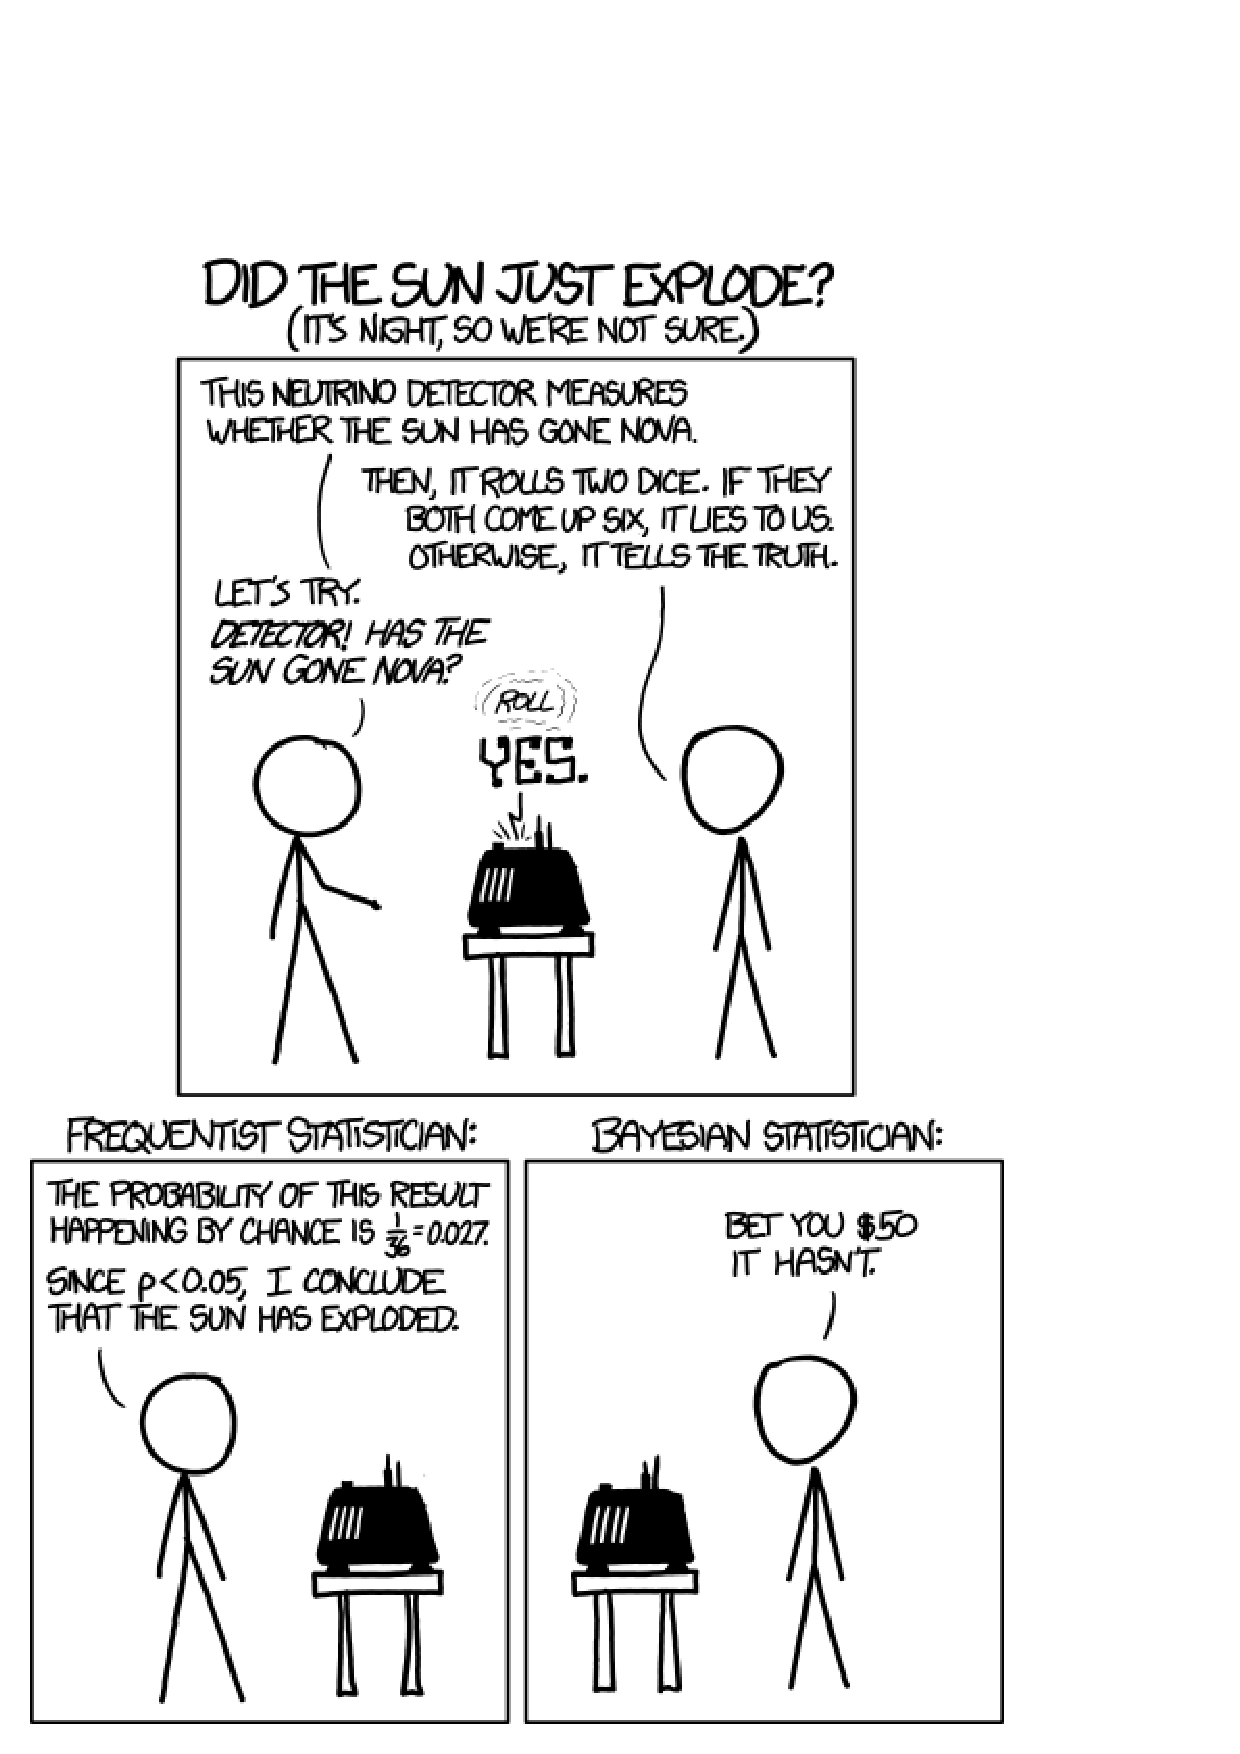
\includegraphics[width=8cm]{frequentists_vs_bayesians.png}
        \else
            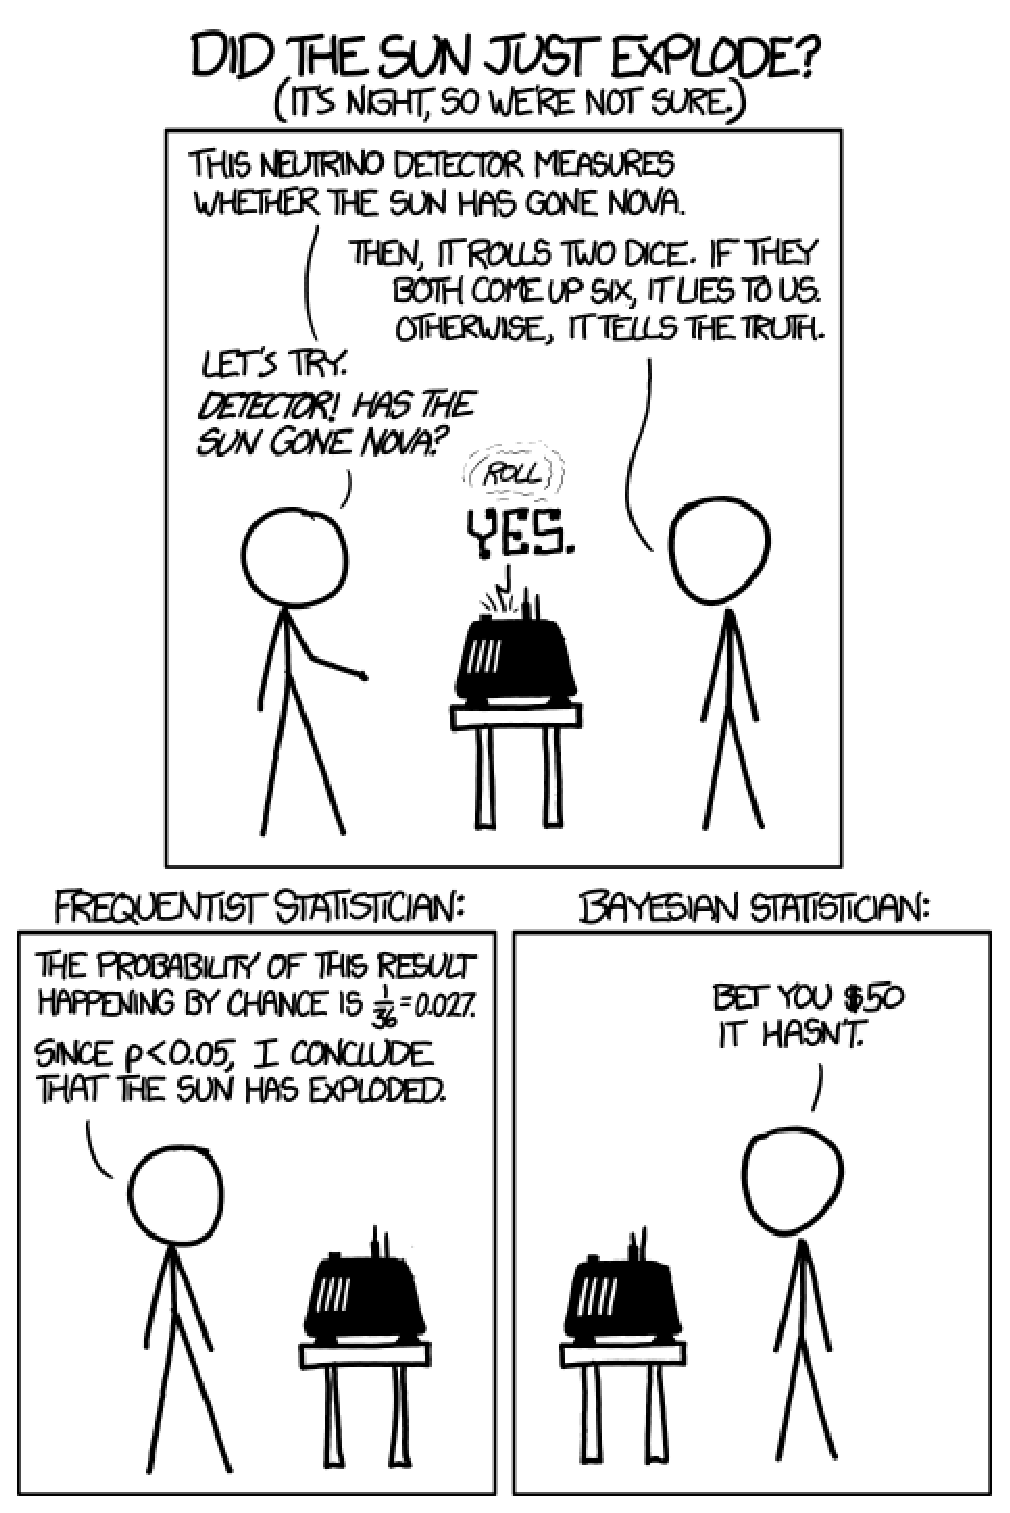
\includegraphics[width=8cm]{frequentists_vs_bayesians.eps}

            \fi

            \url{http://xkcd.com/1132/}, image publiée sous licence \href{http://xkcd.com/license.html}{CreativeCommons}.

\end{center}



%&=& &=& &=& &=& &=& &=& &=& &=& &=& &=& &=& &=& &=& &=& &=& &=& &=& &=& &=& &=& &=& &=& &=& 
\part{Python}
%&=& &=& &=& &=& &=& &=& &=& &=& &=& &=& &=& &=& &=& &=& &=& &=& &=& &=& &=& &=& &=& &=& &=& 
% This is part of Un soupçon de mathématique sans être agressif pour autant
% Copyright (c) 2012
%   Laurent Claessens
% See the file fdl-1.3.txt for copying conditions.

\chapter{Structures de base}

\begin{remark}
    Certains bouts de codes donnés ici commencent par la ligne
    \begin{quote}
        \info{\# -*- coding: utf8 -*-}
    \end{quote}
    Si vous savez ce que signifie «\wikipedia{fr}{Utf8}{utf8}», vous devriez deviner à quoi sert cette ligne. Sinon c'est pas grave : vous n'êtes pas \emph{obligés} de l'écrire dans vos programmes, mais c'est une bonne habitude à prendre. Nous en reparlerons peut-être plus tard.
\end{remark}

%---------------------------------------------------------------------------------------------------------------------------
\subsection{La fonction \info{print}}
%---------------------------------------------------------------------------------------------------------------------------

Python ne prend pas d'initiatives. Si vous ne lui demandez pas d'écrire quelque chose, il n'écrira rien. La commande la plus courante\footnote{Bien entendu, python permet de programmer des fenêtres, des boutons et autres boites de dialogue, auquel cas ce ne sera plus la commande \info{print} qui jouera.} pour afficher quelque chose à l'écran est la commande \info{print}. 
\begin{enumerate}
    \item
        Pour afficher la valeur d'une variable \info{a}, mettre \info{print(a)}.
    \item
        Pour afficher un texte (par exemple «bonjour» ), mettre des guillemets : \info{print(``bonjour'')}.
\end{enumerate}
Si vous voulez afficher plusieurs choses, vous les séparez par une virgule.

\lstinputlisting{ex_print.py}

donne

\lstinputlisting[title=Résultat]{res_ex_print.txt}

Notez que les lignes qui commencent par \# ne sont pas prises en compte. Cela permet au programmeur de mettre des notes pour lui-même. N'hésitez pas à en mettre pour rendre votre code plus lisible.

\Exo{Premiere-0037}

%+++++++++++++++++++++++++++++++++++++++++++++++++++++++++++++++++++++++++++++++++++++++++++++++++++++++++++++++++++++++++++
\section{Listes}
%+++++++++++++++++++++++++++++++++++++++++++++++++++++++++++++++++++++++++++++++++++++++++++++++++++++++++++++++++++++++++++

Une liste est une collection ordonnée d'éléments. Elle se définit avec des crochets.

\lstinputlisting{ex_listes.py}

donne

\lstinputlisting[title=Résultat]{res_ex_listes.txt}

Nous pouvons ajouter un élément à une liste en utilisant la \emph{méthode} \info{append}, et retrouver un élément d'une liste par son numéro (attention : python numérote à partie de zéro), en demandant par exemple \info{A[4]} pour l'élément numéro \( 4\) de la liste \info{A}. Cela sera donc le cinquième élément de la liste. Cas spécial : le dernier élément de la liste est le numéro \( -1\).

\lstinputlisting{ex_listes2.py}

donne

\lstinputlisting[title=Résultat]{res_ex_listes2.txt}


\Exo{Premiere-0033}


La multiplication d'une liste par un nombre donne la liste contenant plusieurs fois la liste originale. Nous ajoutons une liste à une autre en utilisant la méthode \info{extend}.


\lstinputlisting{ex_listes3.py}

donne

\lstinputlisting[title=Résultat]{res_ex_listes3.txt}


\Exo{Premiere-0034}

%+++++++++++++++++++++++++++++++++++++++++++++++++++++++++++++++++++++++++++++++++++++++++++++++++++++++++++++++++++++++++++
\section{Quelque mots à propos des fonctions}
%+++++++++++++++++++++++++++++++++++++++++++++++++++++++++++++++++++++++++++++++++++++++++++++++++++++++++++++++++++++++++++

%---------------------------------------------------------------------------------------------------------------------------
\subsection{Choses Basiques}
%---------------------------------------------------------------------------------------------------------------------------

Si un calcul doit être refait plusieurs fois dans un même programme, il est bon d'écrire une fonction qui sera appelée à chaque fois. En python, une fonction se déclare avec le mot-clef \info{def} comme ceci :
\begin{quote}
    \info{def\ nom\_de\_ma\_fonction(a,b):}
\end{quote}
où \info{a} et \info{b} seront les arguments de la fonction. Il peut y en avoir un seul, deux, ou plus (pas de limites), ou pas du tout. Une fonction peut afficher et calculer autant de résultats intermédiaires que l'on veut. 

\lstinputlisting{ex_fonction.py}

donne

\lstinputlisting[title=Résultat]{res_ex_fonction.txt}

Cette fonction ne fait qu'afficher du texte, mais ne retourne pas de valeurs. Voici une fonction qui retourne \( 1\) si le nombre donné est plus grand ou égal à zéro et retourne \( -1\) si il est négatif.


\lstinputlisting{ex_fonction2.py}

donne

\lstinputlisting[title=Résultat]{res_ex_fonction2.txt}

%---------------------------------------------------------------------------------------------------------------------------
\subsection{Pour aller plus loin}
%---------------------------------------------------------------------------------------------------------------------------

La fonction de l'exemple précédent peut être simplifiée en sachant que dès que une instruction \info{return} est rencontrée, l'exécution de la fonction est \emph{immédiatement} stoppée et la valeur est retournée. Nous pouvons donc écrire

\lstinputlisting{ex_fonction3.py}

Si le nombre donné est positif, un \info{return} est rencontré à l'intérieur du \info{if}, et l'autre \info{return} n'est jamais rencontré.

D'autre part, une fonction peut vraiment prendre \emph{n'importe quoi} comme argument, y compris des autres fonctions. Dans l'exemple suivant, la fonction \info{evaluation} prend un argument une fonction et un nombre, et retourne la fonction évaluée en ce nombre.

\lstinputlisting{ex_fonction4.py}

donne

\lstinputlisting[title=Résultat]{res_ex_fonction4.txt}


%+++++++++++++++++++++++++++++++++++++++++++++++++++++++++++++++++++++++++++++++++++++++++++++++++++++++++++++++++++++++++++
\section{Moyenne, médiane, quartiles}
%+++++++++++++++++++++++++++++++++++++++++++++++++++++++++++++++++++++++++++++++++++++++++++++++++++++++++++++++++++++++++++
\label{SecZYftar}

%---------------------------------------------------------------------------------------------------------------------------
\subsection{Moyenne}
%---------------------------------------------------------------------------------------------------------------------------

\begin{example}     \label{ExerfDMnv}
    % Note : la liste ci-dessous est codée en dur dans les scripts d'exemples. Si on la modifie, il faut modifier les scripts.
    Un magasin de chaussures a vendu des tailles entre \( 40\) et \( 45\) suivant la distribution suivante :
    \begin{center}
        \begin{tabular}{|l||c|c|c|c|c|c|}
            \hline
            taille \( x_i\)&40&41&42&43&44&45\\
            \hline
            effectifs \( n_i\)&3&5&10&8&2&4\\
            \hline
        \end{tabular}
    \end{center}
    Nous voudrions calculer la moyenne, la médiane et les quartiles de la distribution des tailles de chaussures. Nous allons nous occuper de cela dans les pages qui viennent.
\end{example}
    
    Pour calculer la moyenne d'une liste, nous devons savoir la longueur et la somme de ses éléments. Python fournit cela assez rapidement. Si \info{A} est une liste,
    \begin{enumerate}
        \item
            \info{len(A)} est la longueur de \info{A},
        \item
            \info{sum(A)} est la somme de ses éléments.
    \end{enumerate}
    
\Exo{Premiere-0035}
    
Le programme suivant écrit la moyenne de la liste des tailles de chaussures de l'exemple \ref{exnXIMeL}.

\lstinputlisting{chaussures.py}

%\lstinputlisting{res_chaussures.txt}

%---------------------------------------------------------------------------------------------------------------------------
\subsection{Premier et troisième quartiles}
%---------------------------------------------------------------------------------------------------------------------------

Pour les quartiles, nous nous rappelons que si \( n\) est le nombre de valeurs, alors le rang du premier quartile est le premier entier supérieur à \( n/4\); et le rang du troisième quartile est le premier entier supérieur à \( 3n/4\). Par exemple si il y a \( 15\) données, nous calculons \( 3\times 15/3= 11.25\), et le troisième quartile sera la douzième valeur.


Bien entendu python possède une commande qui retourne le premier entier supérieur à un nombre donné. C'est la commande \info{ceil} du module \info{math}. En pratique :

\lstinputlisting{exemple_ceil.py}

donne 

\lstinputlisting{res_exemple_ceil.txt}
De même la fonction \info{math.floor} retourne le premier entier inférieur à un nombre donné. Par exemple \info{math.floor(3.89)} vaut \( 3\).

La ligne \info{import math} s'appelle «importer le module math», et nous n'en dirons sans doute pas plus sur la notion d'import de module. Le module \info{math} contient encore de nombreuses fonctions mathématiques qui transforment python en une très puissante\footnote{Pour donner une idée, la mémoire disponible sur des calculatrices modernes est à peu près la même que celle qui était disponible sur Apple II au début des années 1980; avec python vous pouvez exploiter toute la mémoire de votre ordinateur, ou de votre téléphone ou de votre tablette ou de quoi que ce soit sur lequel vous avez python.} calculatrice scientifique.


\Exo{Premiere-0036}

\lstinputlisting{premier_quartile.py}

Et voici pour la médiane :

\lstinputlisting{mediane.py}


\Exo{Premiere-0038}

%+++++++++++++++++++++++++++++++++++++++++++++++++++++++++++++++++++++++++++++++++++++++++++++++++++++++++++++++++++++++++++
\section{Suite définie par récurrence} 
%+++++++++++++++++++++++++++++++++++++++++++++++++++++++++++++++++++++++++++++++++++++++++++++++++++++++++++++++++++++++++++

Soit une suite définie par récurrence

\begin{subequations}
    \begin{numcases}{}
    u_0=10\\
    u_{n+1}=2u_n.
    \end{numcases}
\end{subequations}

Nous voudrions pouvoir répondre à deux types de questions :
\begin{enumerate}
    \item
        construire une liste contenant les \( 100\) premiers termes de la suite;
    \item
        savoir quel est le premier terme à dépasser un million.
\end{enumerate}

Avant de se lancer, nous devons nous poser une question de vocabulaire : est-ce que le centième terme de la suite \( u\) est \( u_{100}\) ou \( u_{99}\) ? Le premier terme étant \( u_0\), le centième est bien \( u_{99}\).

\lstinputlisting{recurrence1.py}

donne

\lstinputlisting{res_recurrence1.txt}

Notons que la ligne \info{print(u[100])} plante avec l'erreur \info{list index out of range}, c'est à dire que la liste \info{u} n'a pas d'élément \info{u[100]}, ce qui est normal parce qu'elle contient \( 100\) éléments et que la numérotation commence à zéro.


\Exo{Premiere-0039}


En ce qui concerne la possibilité de trouver le premier élément qui dépasse le million, le programme suivant donne deux méthodes.

\lstinputlisting{recurrence2.py}

donne

\lstinputlisting{res_recurrence2.txt}

Notons que la première méthode donne \( 17\) et la seconde donne \( 18\). Qui a raison ? Le \( 18\) de la seconde méthode est la longueur de la liste construite, donc il indique que le premier terme à passer le million est \( u_{17}\) (vu que le premier terme est \( u_0\), la longueur est toujours un plus grande que le numéro du dernier élément).

La réponse est donc que \( u_{17}\) est le premier élément à être plus grand que un million, mais \( u_{17}\) est le dix-huitième élément de la liste.


%+++++++++++++++++++++++++++++++++++++++++++++++++++++++++++++++++++++++++++++++++++++++++++++++++++++++++++++++++++++++++++
\section{Exercices}
%+++++++++++++++++++++++++++++++++++++++++++++++++++++++++++++++++++++++++++++++++++++++++++++++++++++++++++++++++++++++++++


\Exo{Premiere-0027}



%\part{Autres}
%Cette partie contient des choses vues au lycée mais pas spécialement dans mes classes. Ce sont surtout des choses pompées de première année SVT à l'université de Franche-Comté.

\input{theorie}
\input{rappelsLog}


\section{Exponentielles et logarithmes}
% This is part of Exercices de mathématique pour SVT
% Copyright (c) 2010-2011
%   Laurent Claessens et Carlotta Donadello
% See the file fdl-1.3.txt for copying conditions.




\section{Fonctions et graphes}
\input{TD1.tex}


\section{Limites du côté de l'infini}
\Exo{SVT-0001}
\Exo{TD3-0003}

\section{Limite de suites}
\input{TD3.tex}

\section{Étude de fonctions, première partie}
\Exo{TD2-1}
\Exo{TD2A-2}
\Exo{TD2B_1}       
\Exo{TD2-2}

\section{Étude de fonctions, suite}
\Exo{TD4-0001}
\Exo{TD4-0002}
\Exo{TD4-0003}
\Exo{TD4-0004}
\Exo{TD4-0005}

\section{Intégration}
\input{TD5.tex}

\section{Équations différentielles}
\input{TD6A.tex}

\section{Révisions}
\input{TD_revisions.tex}



\Exo{interro-0002}
\Exo{interro-0003}
\Exo{interro-0004}
\Exo{interro-0005}
\Exo{interro-0007}
\Exo{interro-0008}


\Exo{DS2010-1-0001}
\Exo{DS2010-1-0002}
\Exo{DS2010-1-0003}
\Exo{DS2010-1-0004}
\Exo{DS2010-1-0005}

\Exo{DS2010bis-0001}
\Exo{DS2010bis-0002}
\Exo{DS2010bis-0003}
\Exo{DS2010bis-0004}
\Exo{DS2010bis-0005}


\Exo{ExamenDecembre2010-0001}
\Exo{ECdecembre2010-0001}
\Exo{ECdecembre2010-0002}
\Exo{ECdecembre2010-0003}
\Exo{ECdecembre2010-0004}
\Exo{ExamenDecembre2010-0002}
\Exo{ExamenDecembre2010-0003}
\Exo{ExamenDecembre2010-0004}
\Exo{ExamenDecembre2010-0005}
\Exo{Exosenvrac-0001} 
\Exo{Exosenvrac-0015}
\Exo{Exosenvrac-0015A}
\Exo{Exosenvrac-0006}
\Exo{Exosenvrac-0009}


\corrChapitre{Corrigés systématiques}

\input{fdl-1.3.tex}

\bibliographystyle{unsrt}           % unsrt fait que la biblio arrive dans l'ordre de citation au lieu de l'ordre alphabétique.
\bibliography{mazhe}

\addcontentsline{toc}{chapter}{Liste des notations}

\printnomenclature

\printindex

\end{document}

\Exo{smath-0089}
\Exo{smath-0090}
\Exo{smath-0091}
\Exo{smath-0092}
\Exo{smath-0093}
\Exo{smath-0094}
\Exo{smath-0095}
\Exo{smath-0096}
\Exo{smath-0097}
\Exo{smath-0098}
\Exo{smath-0099}
\Exo{smath-0100}

LE SUITE POUR 1STMG
--------------------
Fin de la binomiale (2 semaines)
Tableur : tableau d'effectifs et de fréquences  (1 semaine)
Taux d'évolution, évolutions successives    (3 semaines)
suites numériques   (3 semaines)
dérivation  (3 semaines)
troisième degré (1.5 semaines)
stat : écart type et quartiles  (3 semaines)
intervalles de fluctuation et prise de décision (3 semaines)

LA SUITE POUR LES SECONDES
--------------------------

À faire avec les 2nd2 : tableau de signe des fonctions affines.

Commun encore à faire

Volumes (3s) : un sur les petites surfaces dans les cubes et 2 les positions de droites et plans dans l'espace
Fonctions de référence ax+b,x^2, 1/x : tableau de variation et graphes (2s)

Vecteurs (3s)

Expressions algébriques (dissimulées un peu partout)
Équations par dichotomie
second degré : graphe et tableau de variations (2s)
Inéquations : tableau de signe de produits (1s)
Configurations du plan 
Équations de droites (2s)
Échantillonnage (2s)
Probabilités (2s)
Trigonométrie
